\documentclass[a4paper, 12pt]{ctexart}

% ========== 常用宏包 ==========
\usepackage{geometry} % 页面设置
\geometry{left=2.5cm, right=2.5cm, top=2.5cm, bottom=2.5cm}
\usepackage{amsmath, amsfonts, amssymb} % 数学公式
\usepackage{graphicx} % 插入图片
\usepackage{booktabs} % 三线表
\usepackage{float} % 图片表格浮动位置设置
\usepackage{caption} % 图表标题
\usepackage{color} % 颜色
\usepackage{setspace} % 行距
\usepackage{hyperref} % 超链接与目录
\hypersetup{
    colorlinks=true,
    linkcolor=black,
    filecolor=black,      
    urlcolor=blue,
    citecolor=black,
}

% ========== 文档开始 ==========
\begin{document}

% 标题
\begin{center}
    {\zihao{2} \textbf{共享单车站点智能调度优化问题}} \\[1ex]
\end{center}

% 摘要与关键词
\begin{abstract}
\setstretch{1.2}
（摘要为论文精华，约 300–500 字。须独立成篇，简明扼要地概括：研究问题、所用方法/模型、主要结论和数字结果。评委首先阅读摘要，请务必认真撰写。摘要中不应出现公式，不引用参考文献。）

\vspace{1ex}
\noindent \textbf{关键词：} 关键词1；关键词2；关键词3；关键词4（3–5 个，以分号分隔）
\end{abstract}

% 目录页
\newpage
\tableofcontents
\newpage

\setstretch{1.25} % 正文行距

% ========== 正文部分 ==========

\section{问题重述}

\subsection{问题背景}
近年来，共享单车已深度融入宁波市大学城居民的日常生活。由于校园周边群体作息高度规律，单车使用呈现出显著的早晚高峰 “ 潮汐现象 ” 。教学区、交通枢纽等热门站点极易面临无车可借的窘境，而偏远站点则出现车辆严重积压。这种供需在时空上的错配不仅降低了运营效率，还极大地影响了用户的出行体验。现有的纯人工经验调度模式成本高昂，且难以实现单车在时间、空间和数量上的精准匹配。

\subsection{核心问题}
本项目旨在利用提供的大学城单车站点基础信息与长达一周的每小时借还历史数据，挖掘单车需求的时空演变与潮汐规律。在此基础上，综合考虑空 / 满桩惩罚成本、单车运输及装卸人工成本，构建科学的运筹优化调度模型，从而为大学城制定低成本、高效率且能最大化满足用户出行需求的智能化单车调度策略。

\section{问题分析}

本题的核心目标是通过挖掘共享单车历史借还数据的时空分布规律，预测未来需求，并据此制定成本最小化的车辆智能调度策略。问题层层递进，从描述性统计分析到需求预测，再到运筹优化与敏感性检验。以下是对各子问题的详细解题思路与方法选择依据的分析：

\subsection{问题一}
本问题旨在通过对附件 2 中时序数据的探索性数据分析，挖掘宁波大学城区域站点的日借还规律。为了保证分析的科学性与结论的鲁棒性，我们将该问题拆解为三个子维度进行逐一攻克：

\textbf{（1）针对典型高峰时段及其持续时长的识别：}
原始的每小时借还数据不可避免地存在随机波动（噪音）。为了精准捕捉趋势，我们首先采用 3 小时中心移动平均法对全天时间序列进行平滑处理。此外，考虑到周末或非核心站点的单车日吞吐量绝对值极低，如果仅采用分位数来判定高峰，极易陷入“分位数陷阱”（即将基数极小的波动误判为高峰）。因此，我们设计了“相对分位数（$Q_{0.8}$）+ 绝对全局均值（$\mu$）”的双重阈值判定法，只有同时突破这两道阈值的时段才被认定为真实高峰，随后将相邻的高峰小时进行合并以提取持续时长。

\textbf{（2）针对极端站点及其时空分布特征的挖掘：}
极热（Top 5）与极冷（Bottom 5）站点的供需极度不平衡是导致单车积压或无车可借的根源。我们首先根据全周总借出量筛选出这两类极端站点。在时间特征上，我们引入绝对/相对峰值强度与潮汐相位不对称性等指标，量化其时间维度的需求错位；在空间特征上，纯粹的经纬度散点图缺乏业务解释力，因此我们引入了外部的高德/百度地图兴趣点（Point of Interest，POI）数据以及局部站点密度指标，从宏观功能分区与微观设施配套两个层面，定性与定量结合地剖析极端站点的空间集聚特征。

\textbf{（3）针对工作日与休息日借还模式的差异对比：}
工作日与休息日由于人群作息的不同，必然在共享单车的使用上呈现异质性。我们采用“宏观城市级+微观站点级”的双重视角。在城市级别，对比两大类日期的整体均值、极值与变异系数，并引入独立样本 Mann-Whitney U 非参数检验，从统计学层面严格验证二者分布形态的显著差异；在站点级别，选取热、冷及中等热度的代表性站点，重点考察休息日早高峰是否出现符合常理的“时间推迟”现象。

\subsection{问题二}
本问题要求建立未来 24 小时各站点每小时借还量的需求预测模型。
由于共享单车的借还需求表现出高度的非线性、明显的周期性（以天/周为单位）以及复杂的时空耦合特征（站点间的距离与功能区相似性会相互影响），传统的线性时序模型（如 ARIMA）难以捕捉这些复杂关系。因此，我们将考虑引入具备时序记忆能力与特征捕捉能力的机器学习或深度学习模型（如随机森林、LightGBM 或基于 LSTM 的序列预测模型）。模型将以第一问中提取的时空特征（如星期特征、历史平滑借还量、站点周边 POI 属性）作为输入，以附件 2 的前 6 天数据为训练集，最后一天（周日）为测试集进行预测与精度评估。

\subsection{问题三}
本问题是整个赛题的核心，要求基于预测的需求结果建立单车调度优化模型。
这本质上是一个带有容量限制与软时间窗约束的车辆路径规划问题（VRP）的复杂变体。我们的决策变量包括调度货车的行驶路线、在各站点的装卸数量以及到达时间。目标函数是最小化系统总成本（即货车的距离运输成本、单车的装卸人工成本以及由于时空错配导致的满桩/空桩惩罚成本）。
针对整点计算惩罚成本的约束，我们将构建一个离散时间的混合整数线性规划（MILP）模型。若模型规模较小，可尝试使用 Gurobi/CPLEX 等求解器进行精确求解；若因状态空间爆炸导致求解困难，我们将设计启发式算法（如遗传算法或模拟退火算法）以在合理时间内寻找近似最优调度策略，并与无调度情况下的各项指标进行全面对比。

\subsection{问题四}
本问题要求对前述调度模型进行空间网络上的推广与核心成本参数的灵敏度分析。
首先，针对新增的 5 个站点，我们将依据第一问中发现的空间聚集规律（如选择 POI 密集且当前缺乏站点的盲区）自主设定其坐标与容量，并将其作为新节点无缝接入问题三建立的图网络拓扑中，重新运行调度模型以验证算法的普适性。其次，针对单变量（如运输单价、惩罚系数），我们将采用控制变量法，通过设定不同的参数梯度，观察目标函数值与最优调度路线的演化路径，进而为共享单车运营方提供在不同成本结构下的动态策略调整建议。

\section{模型假设}
为确保数学模型的科学性与求解的严谨性，本文基于赛题数据与实际业务场景，提出以下合理假设：

\begin{description}
    \item[假设一：时间颗粒度与后延规则。] 统一使用时间后延规则，时间颗粒度设为 1 小时（如“0”表示 00:00 - 00:59）。假定若某单一小时内出现借出或归还量峰值，而其相邻的两个小时数据处于较低水平，则认定该高峰持续时间为 1 小时。此设定与附件 2 提供的数据精度完全契合。
    
    \item[假设二：时空特征语义化分段。] 为增强后续规律提取的可解释性，在时间维度上，假定可将全天划分为凌晨（1-5）、早晨（6-10）、中午（11-13）、下午（14-16）、傍晚（17-19）、夜晚（20-22）与午夜（23-0）七个业务语义时段；在空间维度上，假定针对研究区域（东经 $121.4637^\circ \sim 121.9966^\circ$，北纬 $29.7738^\circ \sim 29.9605^\circ$）内的站点，可通过外部查阅权威地图资料获取的 POI 数据，客观辅助划分为商业区、居住区、文教区等功能性分区，以避免纯主观臆断。
    
    \item[假设三：平滑处理的边界截断。] 在对时序数据使用中心移动平均法进行平滑降噪时，针对该周起始与结束的若干小时内因数据不足无法套用滑动窗口的情况，假定一律保留原始数据。其合理性在于：午夜至凌晨时段几乎不可能成为共享单车的借还高峰，因此不对边界数据进行平滑处理实际上不会对全局高峰时段的识别结果产生干扰。
    
    \item[假设四：无外部特殊事件干扰。] 经查阅日历，2025 年 4 月 7 日至 4 月 13 日期间无中国法定节假日。因此假定该周内共享单车的供需规律仅受常规的“工作日”与“休息日”两种通勤模式主导，不存在节假日调休效应或极端恶劣天气等不可抗力的突发干扰。
\end{description}

\section{符号说明}

\begin{table}[H]
    \centering
    \caption{主要数学符号及其含义}
    \begin{tabular}{ccc}
        \toprule
        \textbf{符号} & \textbf{含义说明} & \textbf{单位/备注} \\
        \midrule
        $d, h, s$ & 决策与统计的索引：天、小时、站点的序号 & 离散整数 \\
        $B^{total}_{d, h}$ & $d$日$h$时所有站点的借出量总和 & 辆 \\
        $R^{total}_{d, h}$ & $d$日$h$时所有站点的归还量总和 & 辆 \\
        $\tilde{B}^{total}_{d, h}$ & 经过3小时中心移动平均平滑后的借出总量 & 辆 \\
        $Q_{0.8}(\cdot)$ & 时间序列的 80\% 分位数阈值 & 辆 \\
        $\mu_{B}, \mu_{R}$ & 全周全部时间段内借出与归还数据的全局均值 & 辆 \\
        \bottomrule
    \end{tabular}
\end{table} 

\section{数据说明} 
为全面剖析单车借还规律并建立调度模型，本文主要依赖以下结构化数据与外部辅助地理数据（数据涵盖2025年4月7日至4月13日）：
\begin{itemize}
    \item \textbf{站点基础属性数据（附件1）}：包含大学城及周边区域各共享单车站点的唯一编号、名称、地理经纬度坐标、总桩位容量及期初库存量。该数据为构建空间网络拓扑图和计算站间物理距离提供了基础地理特征。
    \item \textbf{站点时序借还数据（附件2）}：记录了上述站点在7天内、每天24小时粒度下的借出量与归还量。该数据集是捕捉用户出行潮汐特征、区分工作日与周末模式、以及进行需求时间序列预测的核心输入。
    \item \textbf{调度约束与成本参数（附件3）}：详尽列出了运筹优化模型的边界条件与目标函数权重。包括货车最大载量（15辆/次）、运输成本（3.5元/公里）、装卸成本（2.0元/辆）、满/空桩惩罚系数、调度车速以及每日合规的调度时间窗等，是构建第三问成本极小化目标函数的直接依据。
    \item \textbf{外部开源 POI 地理数据}：利用 Python 从高德/百度地图接口获取站点周边（100m 核心区及 1km 辐射区）的POI数据，用于客观佐证站点的功能分区属性。
\end{itemize}

\section{数据预处理与特征聚合}
在进行探索性数据分析与运筹建模前，为确保数据的准确性与模型训练的稳定性，本文对原始数据进行了系统性的校验、重构与指标聚合，构建了可供各子问题直接调用的特征底表：

\subsection{异常值与数据完整性检验}
对附件 1 与附件 2 进行系统校验。经 Python Pandas 库核查，本赛题提供的数据质量极佳，不存在缺失值（NaN）与单小时借还量远超站点容量的明显离群点。因此，本文无需进行主观的均值插补，直接保留原始记录以反映最真实的用户需求分布。

\subsection{多源数据联结与特征衍生}
为实现时空联合分析，本文以“站点编号”为主键，将静态地理信息左连接至动态时序表中，并展开时空双维度的特征衍生。在\textbf{时间特征}方面，将日期字段映射为具体的星期标识，生成布尔型特征 Is\_Weekend（工作日记为 0，休息日记为 1），同时将全天划分为凌晨、早晨等 7 个离散时段，以支撑后续的潮汐相位分析。在\textbf{空间特征}方面，预先计算所有站点两两之间的球面距离矩阵以备路径规划之需，并结合 POI 数据衍生出“局部站点密度”特征。

\subsection{多维指标聚合与底表构建}
为了给后续的规律描述与需求预测提供基础的结构化输入，本文在时间与空间两个维度上进行了数据聚合。在\textbf{全局时序指标}层面，对每天 $d$ 每个小时 $h$ 内全部 30 个站点的借出与归还量分别求和，得到全区域维度的时序数据集 $\{B^{total}_{d, h}\}$ 和 $\{R^{total}_{d, h}\}$。在\textbf{站点面板指标}层面，针对空间维度的极端值挖掘需求，预先计算每个站点 $s$ 在整周内的总借出量，生成数据集 $\{B^{total}_{s}\}$ 并持久化存储，以便在后续工作日差异分析及第三问调度模型中跨模块无缝复用。

\section{模型建立与求解}

\subsection{问题一：基于多维时空特征的单车借还规律描述性分析} 

\subsubsection{站点借还高峰时段的识别与特征提取}

真实场景下的共享单车借还需求极易受偶发因素影响，导致原始小时级时序数据存在明显的随机波动。为了精准提取真实的潮汐趋势，本文首先对数据进行降噪处理，随后提出了一种双重阈值判定法来锁定典型高峰时段。

\textbf{1. 时序数据的平滑降噪}

对每天 $d$ 的每个小时 $h$ 内大学城 30 个站点的借出与归还数量分别求和，得到全量数据集 $\{B^{total}_{d, h}\}$ 和 $\{R^{total}_{d, h}\}$。为减小高频噪音对高峰识别的干扰，使峰值区间的变化更符合出行惯性，本文采用 3 小时中心移动平均法进行平滑处理。以借出总量为例，平滑后的数值 $\tilde{B}^{total}_{d, h}$ 计算如下：
$$
\tilde{B}_{d,h}^{total} = 
\begin{cases} 
\frac{1}{3}(B_{d,h-1}^{total} + B_{d,h}^{total} + B_{d,h+1}^{total}), & h \neq 23 \\ 
\frac{1}{3}(B_{d,h-1}^{total} + B_{d,h}^{total} + B_{d+1,0}^{total}), & h = 23 
\end{cases}
$$
同理可得到平滑后的归还总量 $\tilde{R}^{total}_{d, h}$。对于该周绝对起始与结束的小时，因数据不足以支撑滑动窗口，根据模型假设，本文一律保留原始数据。

\textbf{2. 双重阈值高峰判定模型}

在提取高峰时，若仅使用单一的分位数标准，极易在总体单车吞吐量极低的低谷日（如周末或恶劣天气）强行框选出并不具备绝对业务意义的高峰（即“分位数陷阱”）。为此，本文构建了“相对分位数 + 绝对全局均值”的双重阈值判定法（以借出峰为例）：

首先，分别计算单日 24 小时序列的 80\% 分位数阈值 $Q_{0.8}(\tilde{B}^{total}_{d, h})$，并计算整周所有时段数据的全局均值 $\mu_B$ 作为绝对下限。当且仅当 $d$ 日 $h$ 时满足以下条件时，方可被记为借出高峰小时：
$$
\tilde{B}^{total}_{d, h} \geq \max \left( Q_{0.8}(\tilde{B}^{total}_{d, h}), \mu_B \right)
$$
随后，算法将相邻的高峰小时进行合并，生成连续的高峰时段及其持续时长。图 \ref{fig:methodology} 选取了典型工作日直观演示了该方法在单日时序序列上的截断与判定过程。

\begin{figure}[H]
    \centering
    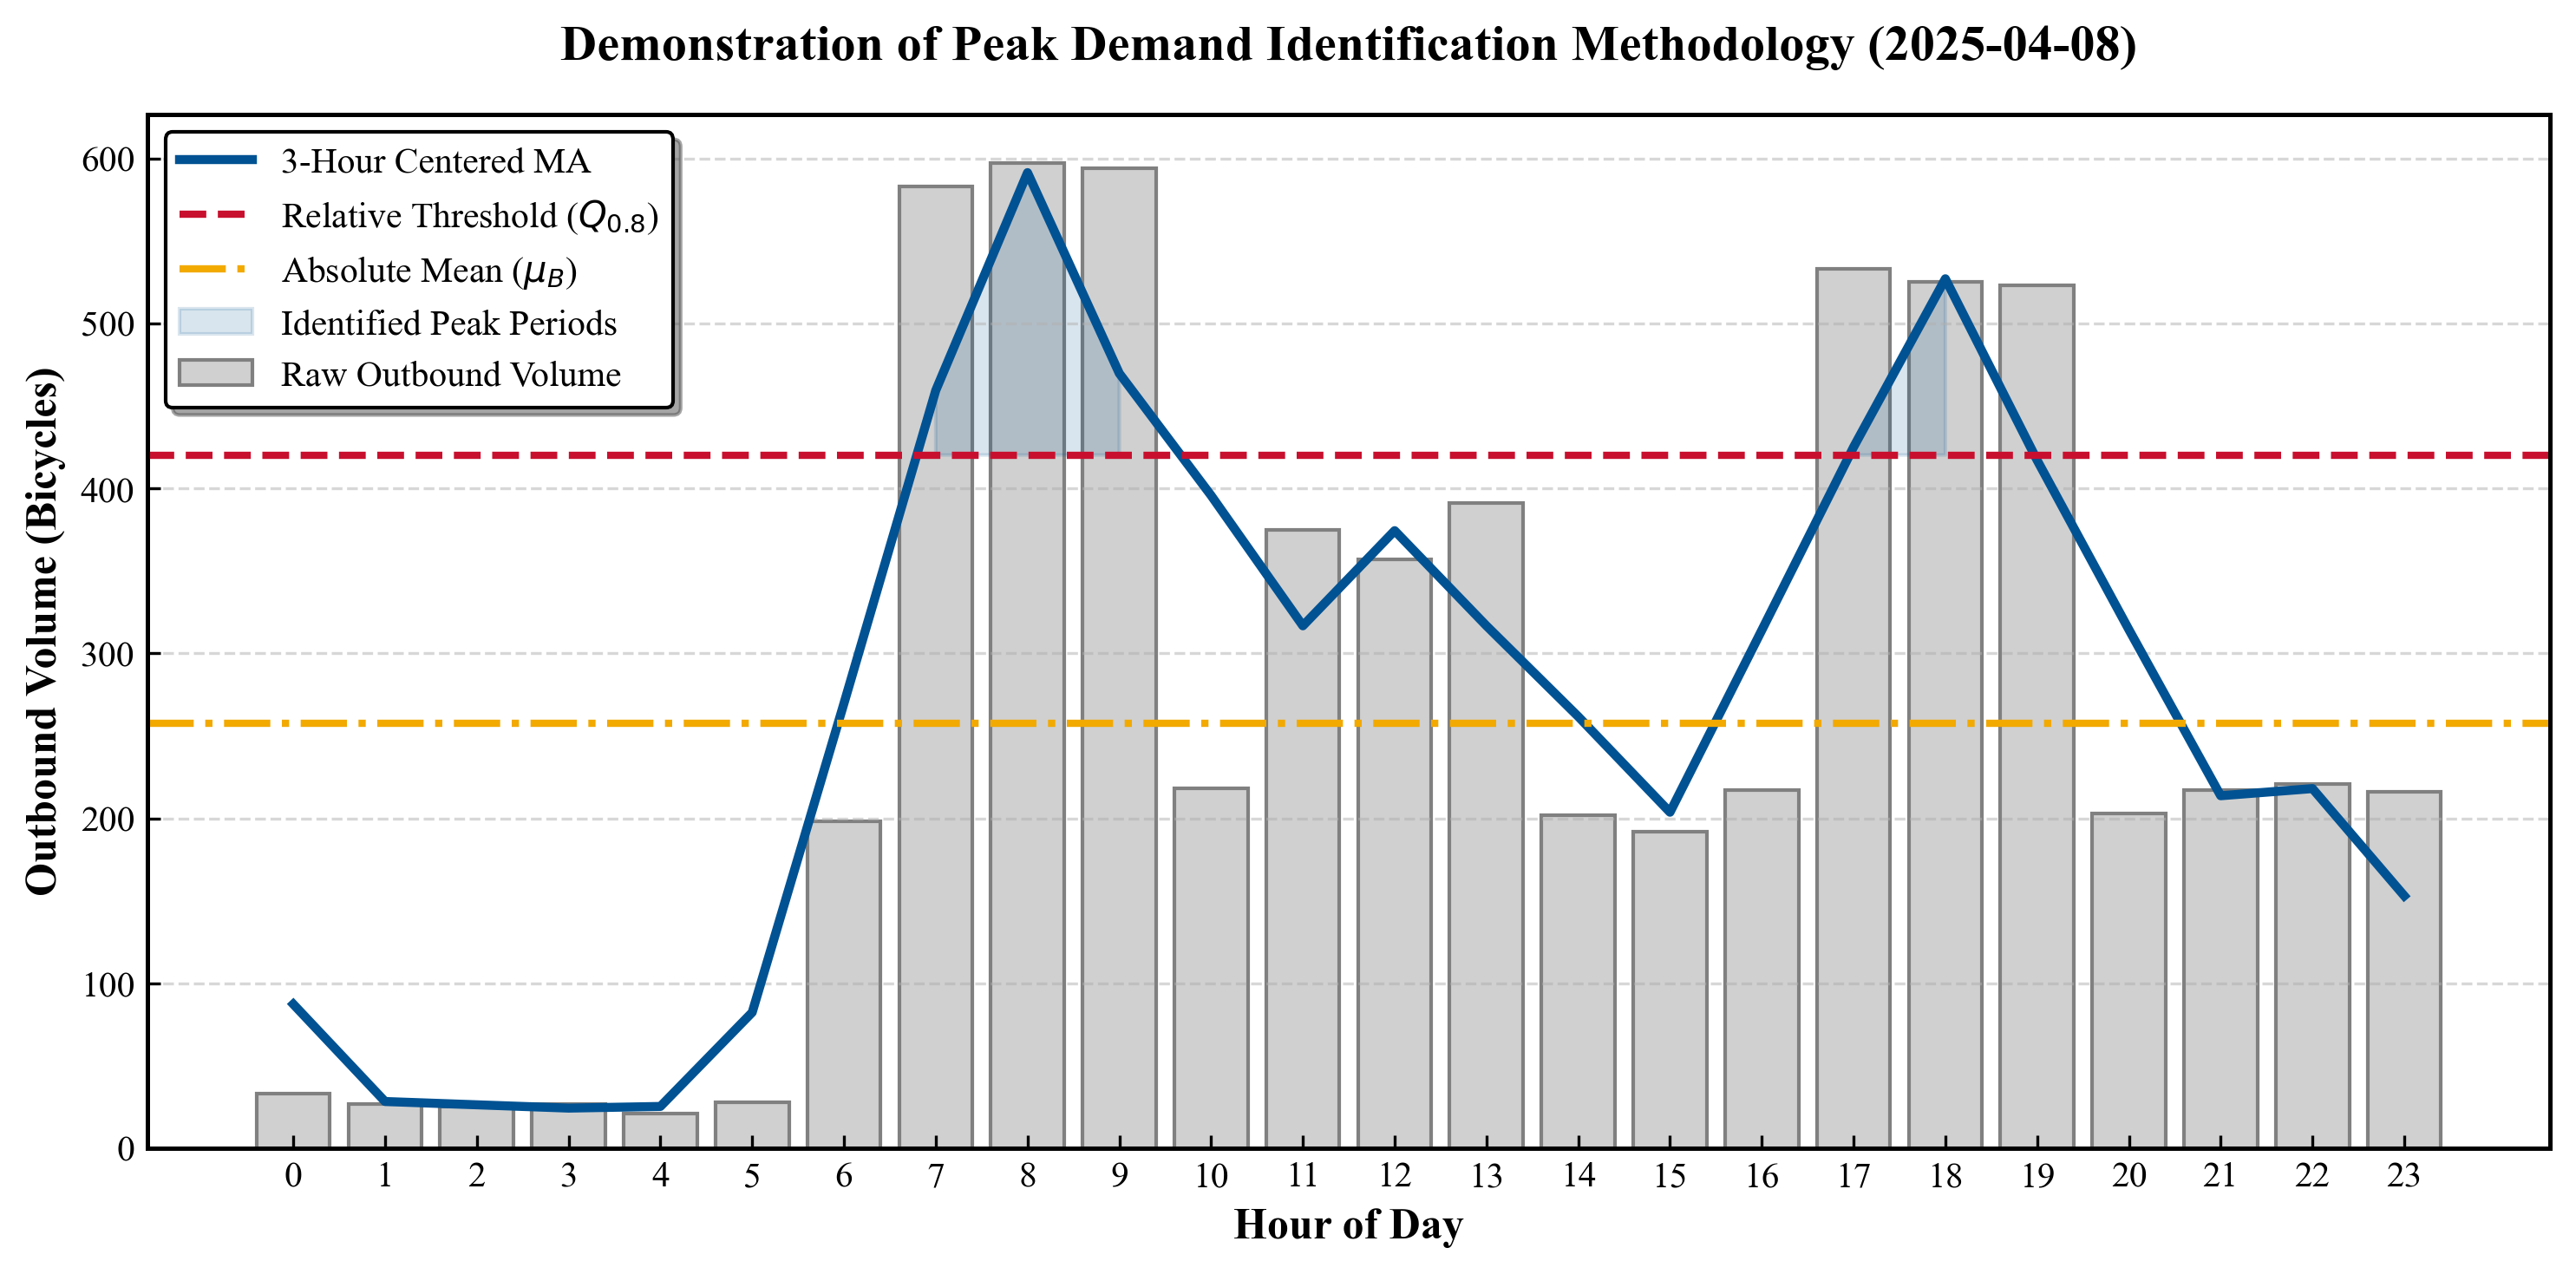
\includegraphics[width=0.9\textwidth]{Fig1_Methodology.png} 
    \caption{单车借还高峰双重阈值判定方法论演示（以某典型工作日为例）}
    \label{fig:methodology}
\end{figure}

\textbf{3. 结果提取与业务规律总结}

基于上述模型对全周数据进行遍历处理，本文首先绘制了全周单车借出需求的时空潮汐热力图（如图 \ref{fig:peak_heatmap} 所示）。

\begin{figure}[H]
    \centering
    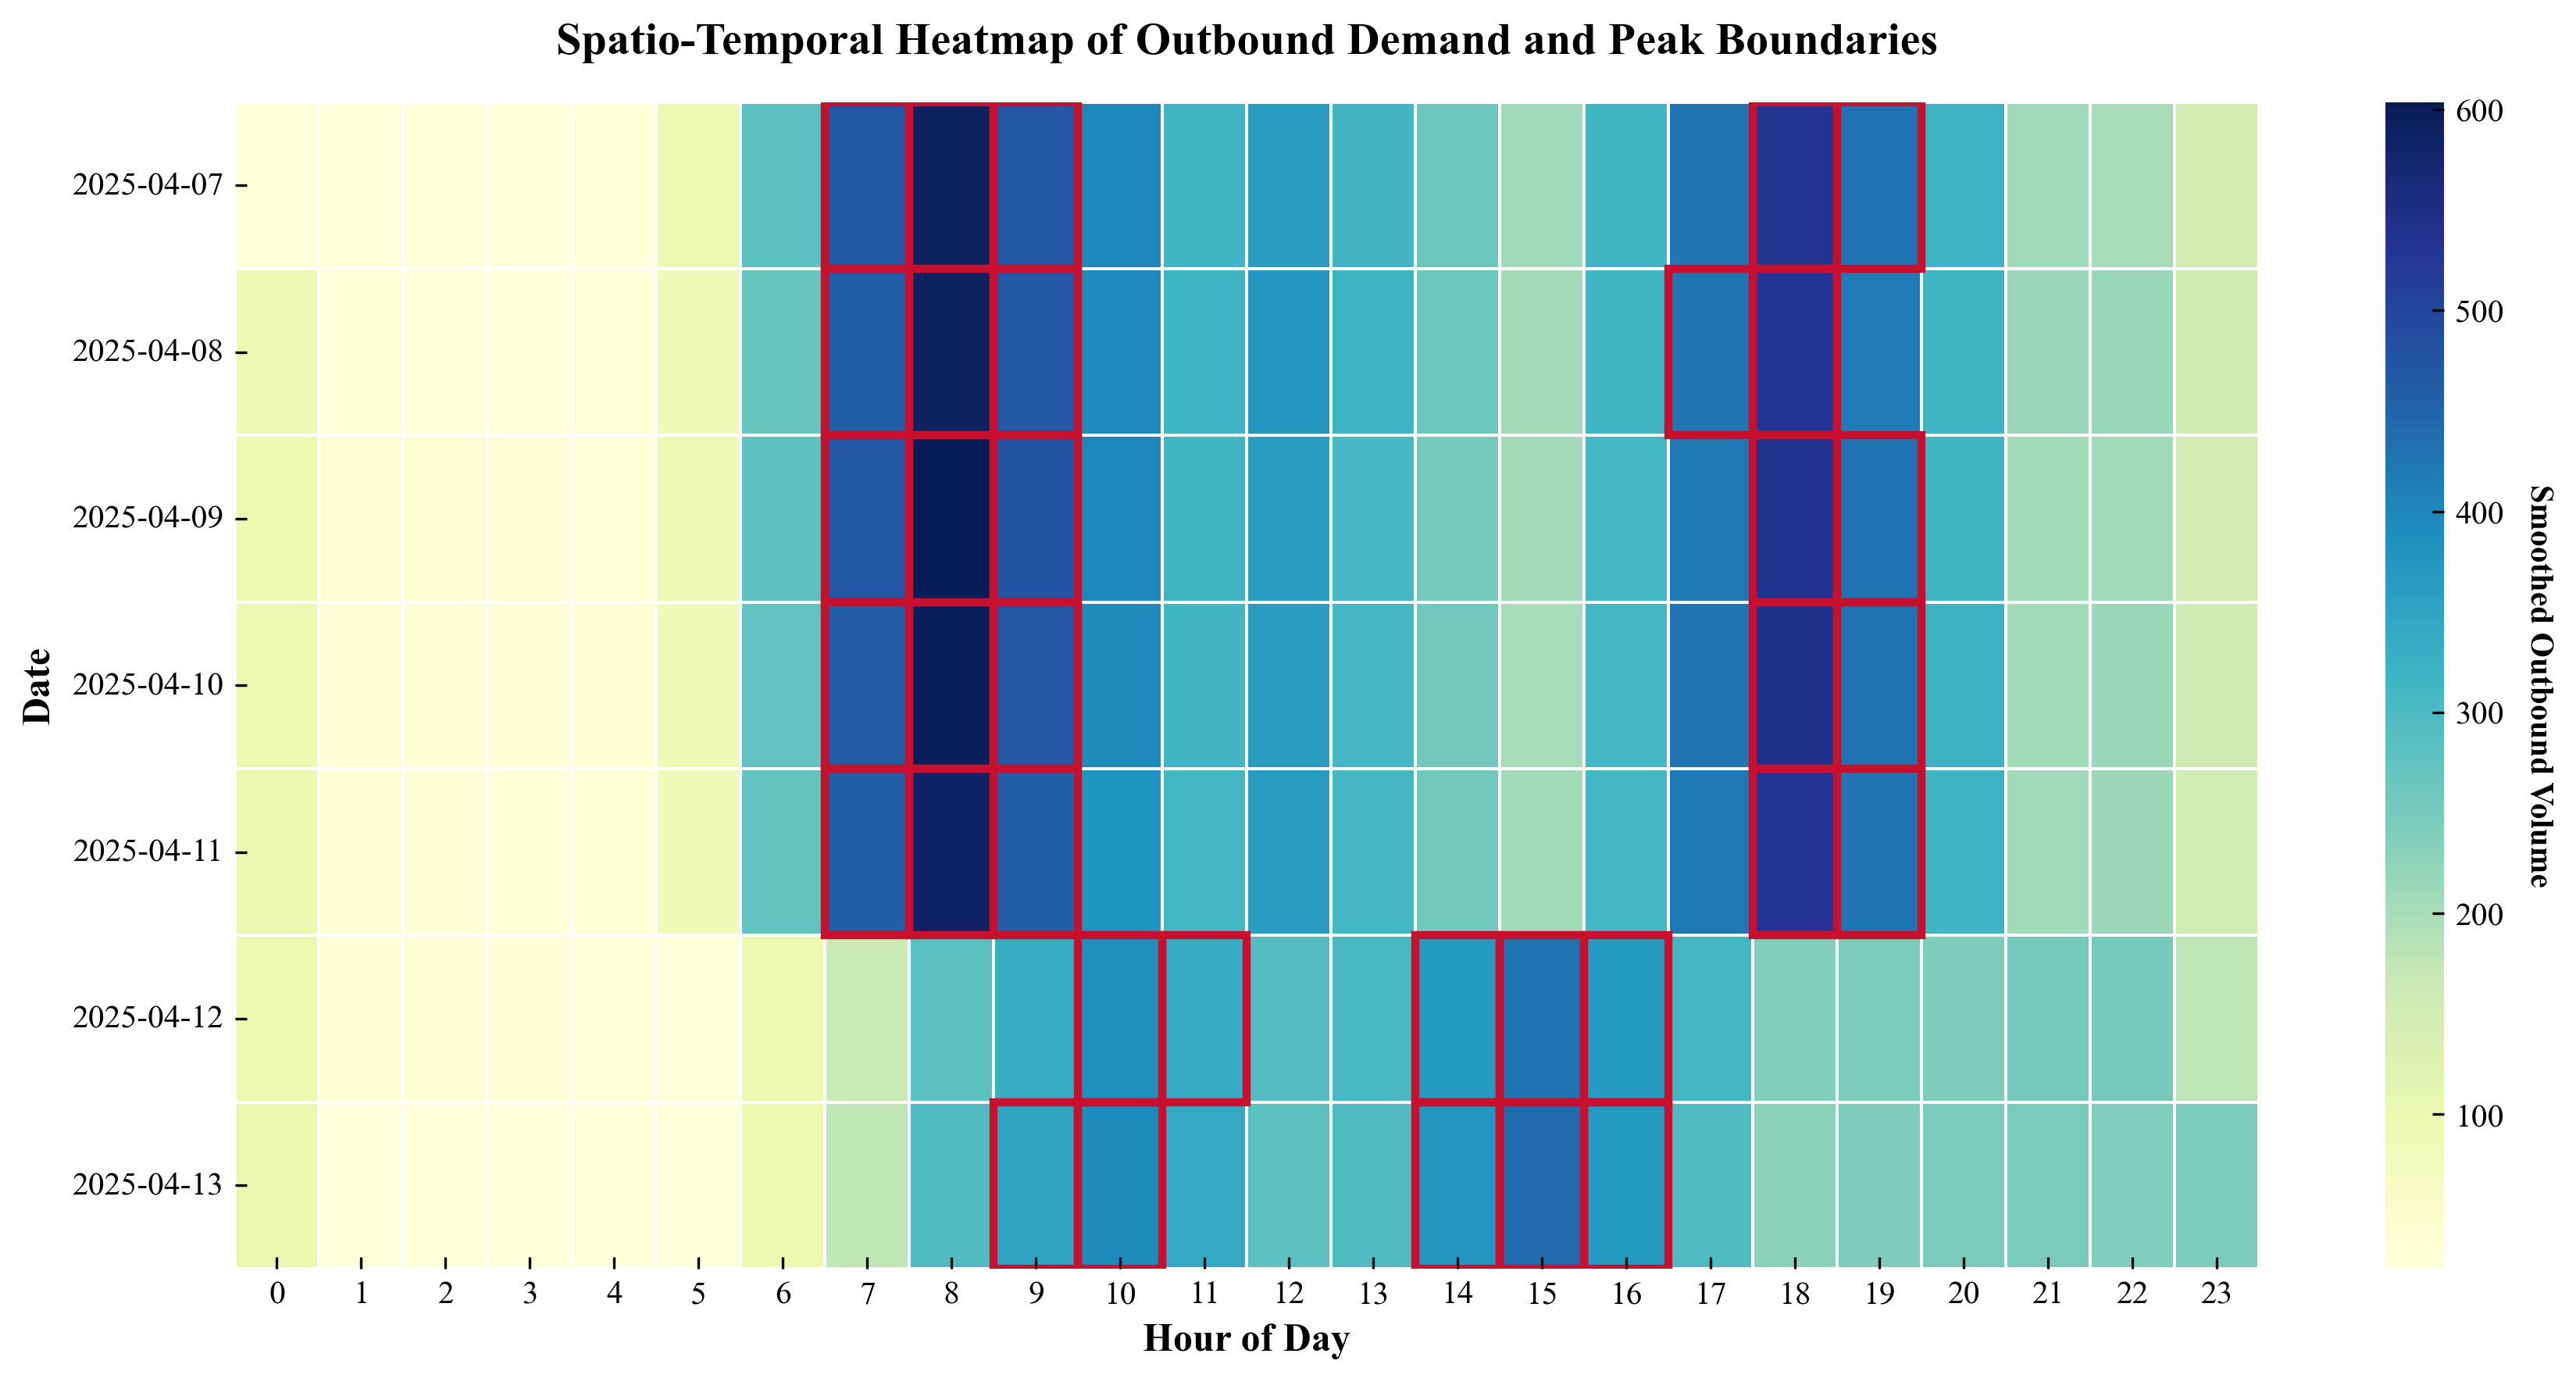
\includegraphics[width=0.9\textwidth]{Fig2_Heatmap.png} 
    \caption{全周单车借出需求时空热力分布及高峰边界}
    \label{fig:peak_heatmap}
\end{figure}

通过热力图的高亮边界可以直观看出，特定时段内的借还需求并非平缓过渡，而是呈现爆发式聚集，时空错配现象极大地加剧了供需矛盾。为了进一步量化这种聚集效应在全天 24 小时上的分布特征，本文统计了被严格判定为“借出高峰”的时段频数（如图 \ref{fig:peak_dist} 所示）。

\begin{figure}[H]
    \centering
    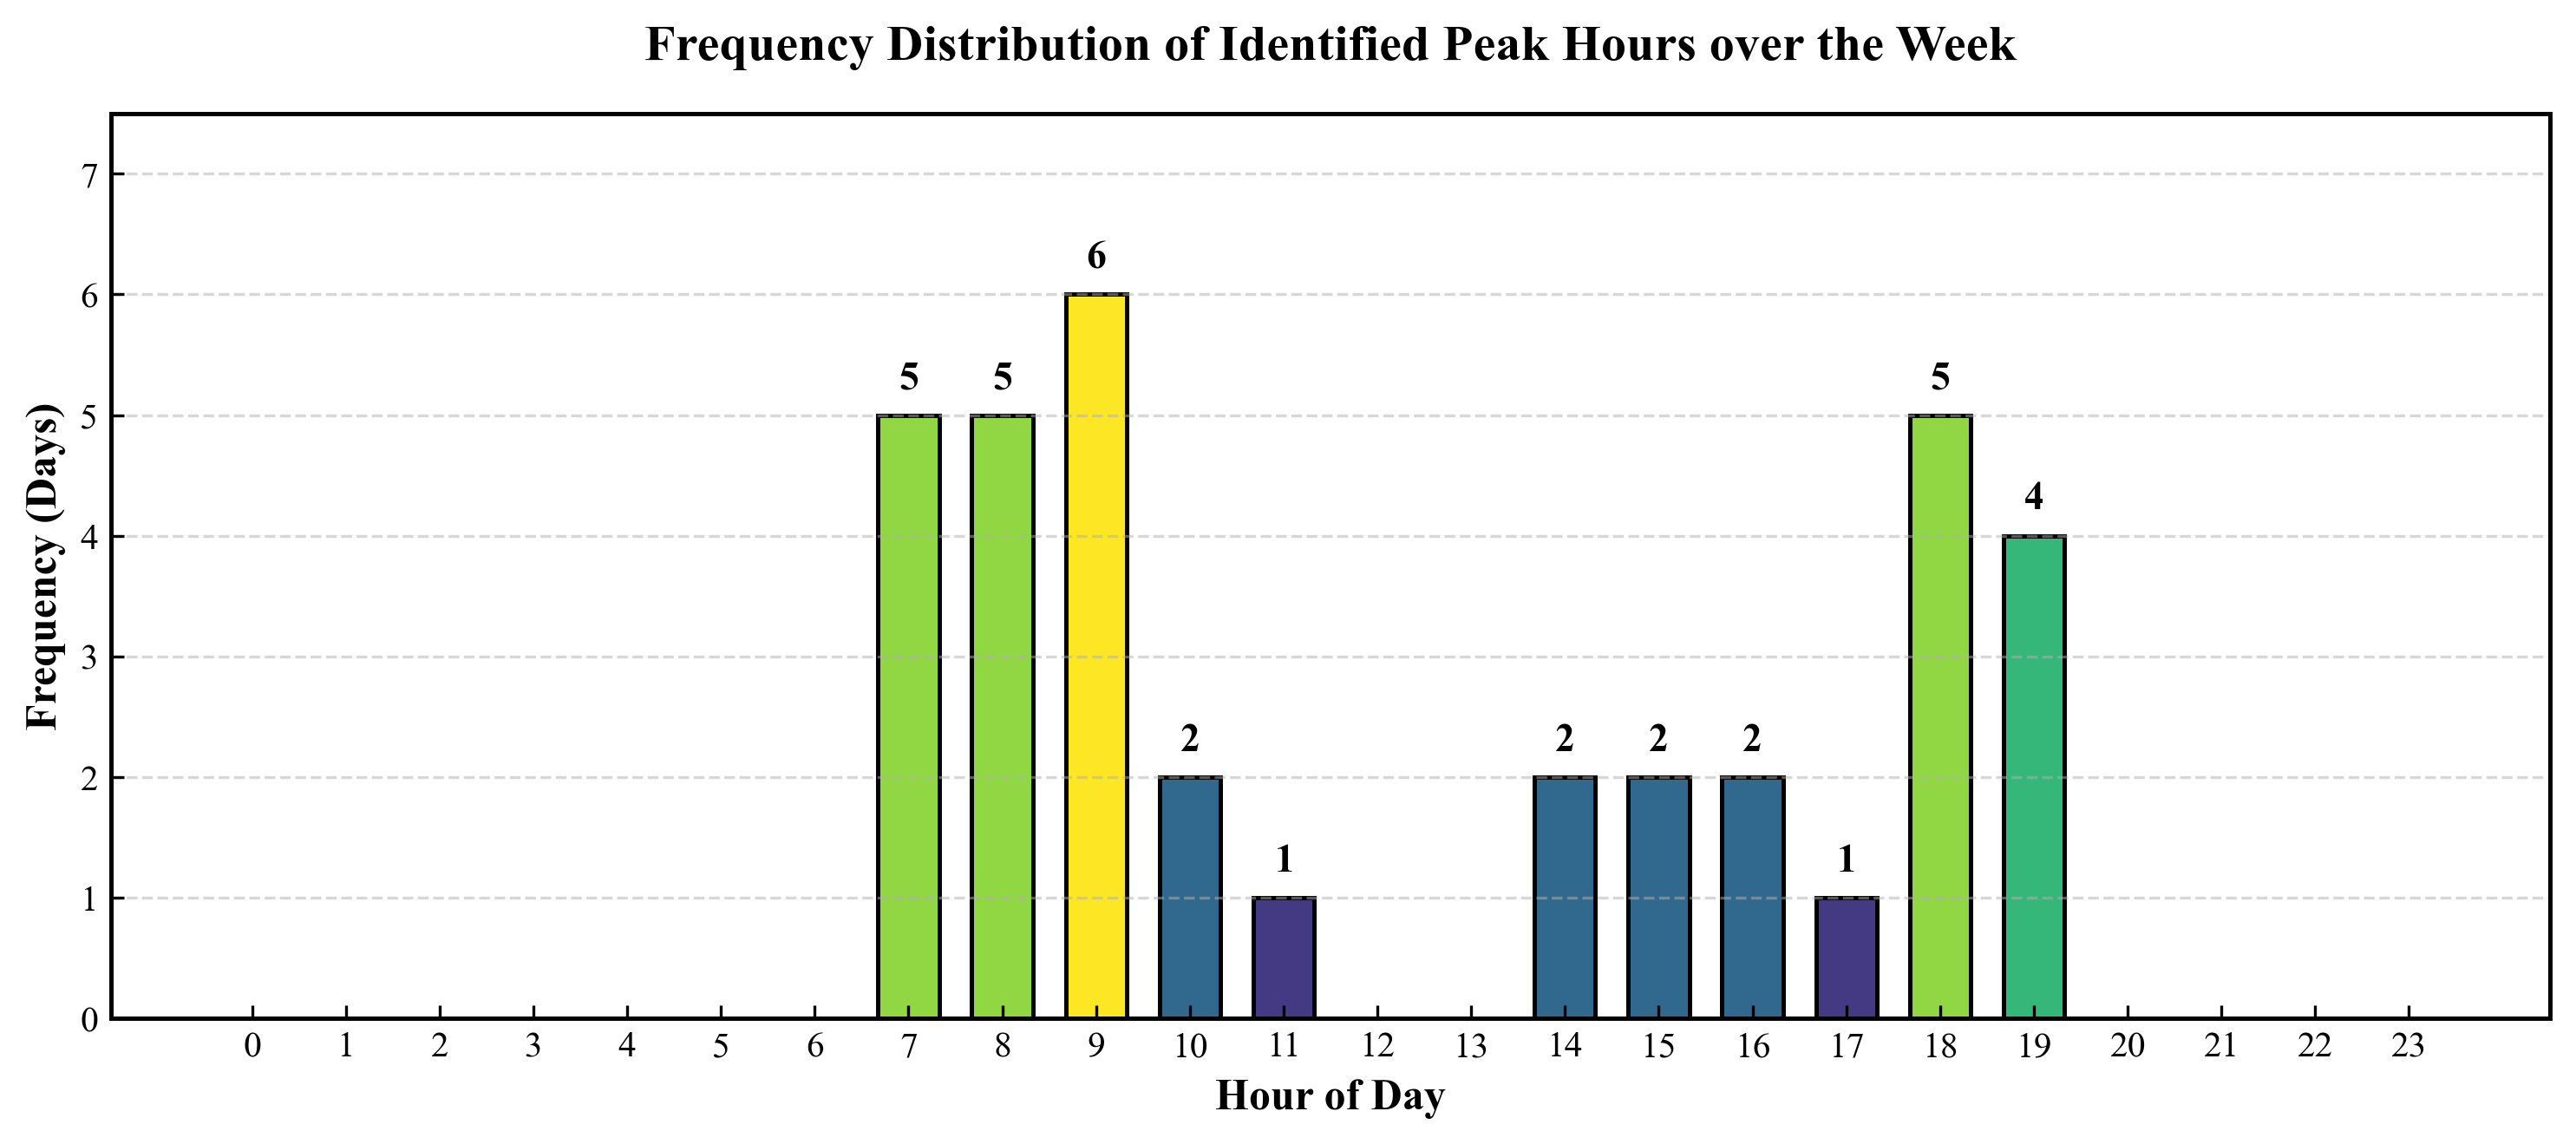
\includegraphics[width=0.9\textwidth]{Fig3_Peak_Frequency.png} 
    \caption{全周被判定为“借出高峰”的时段频数分布}
    \label{fig:peak_dist}
\end{figure}

综合上述图表的深度剖析，可提炼出以下核心业务规律：大学城区域的单车需求存在极其显著的\textbf{“双峰潮汐特征”}。借出与归还高峰高度集中在早晨（7:00-9:00）与傍晚（17:00-19:00）两个核心时间段。这与师生群体“早晨从宿舍区前往教学区或交通枢纽，傍晚逆向返回”的通勤作息完美吻合，每次典型高峰的平均持续时长约为 2 至 3 小时。

本节提取出的典型高峰时段与极端的潮汐特征，精准刻画了运营系统的承载瓶颈。这不仅将为问题二的需求序列预测提供至关重要的周期性先验输入，更为问题三中决定“何时出车调度”以及评估满桩/空桩惩罚成本奠定了坚实的事实与数据依据。

\paragraph{稳健性检验：平滑窗口尺度与降噪机制} 

在上述时间序列特征提取过程中，3 小时中心移动平均平滑与双重阈值的配合虽能有效揭示宏观规律，但仍需警惕特定算法参数带来的过拟合风险。为验证本节提取的高峰时段并非由特定的“3 小时平滑窗口”这一超参数偶然促成，本文进行了严格的方法学稳健性检验。

本文分别将模型退化为“无平滑处理（保留原始时序）”以及扩展为“5 小时中心移动平均平滑”，在相同双重阈值体系下重新执行高峰判定，并生成了不同平滑尺度下的高峰判定差异矩阵（如图 \ref{fig:robustness} 所示）。

\begin{figure}[H]
    \centering
    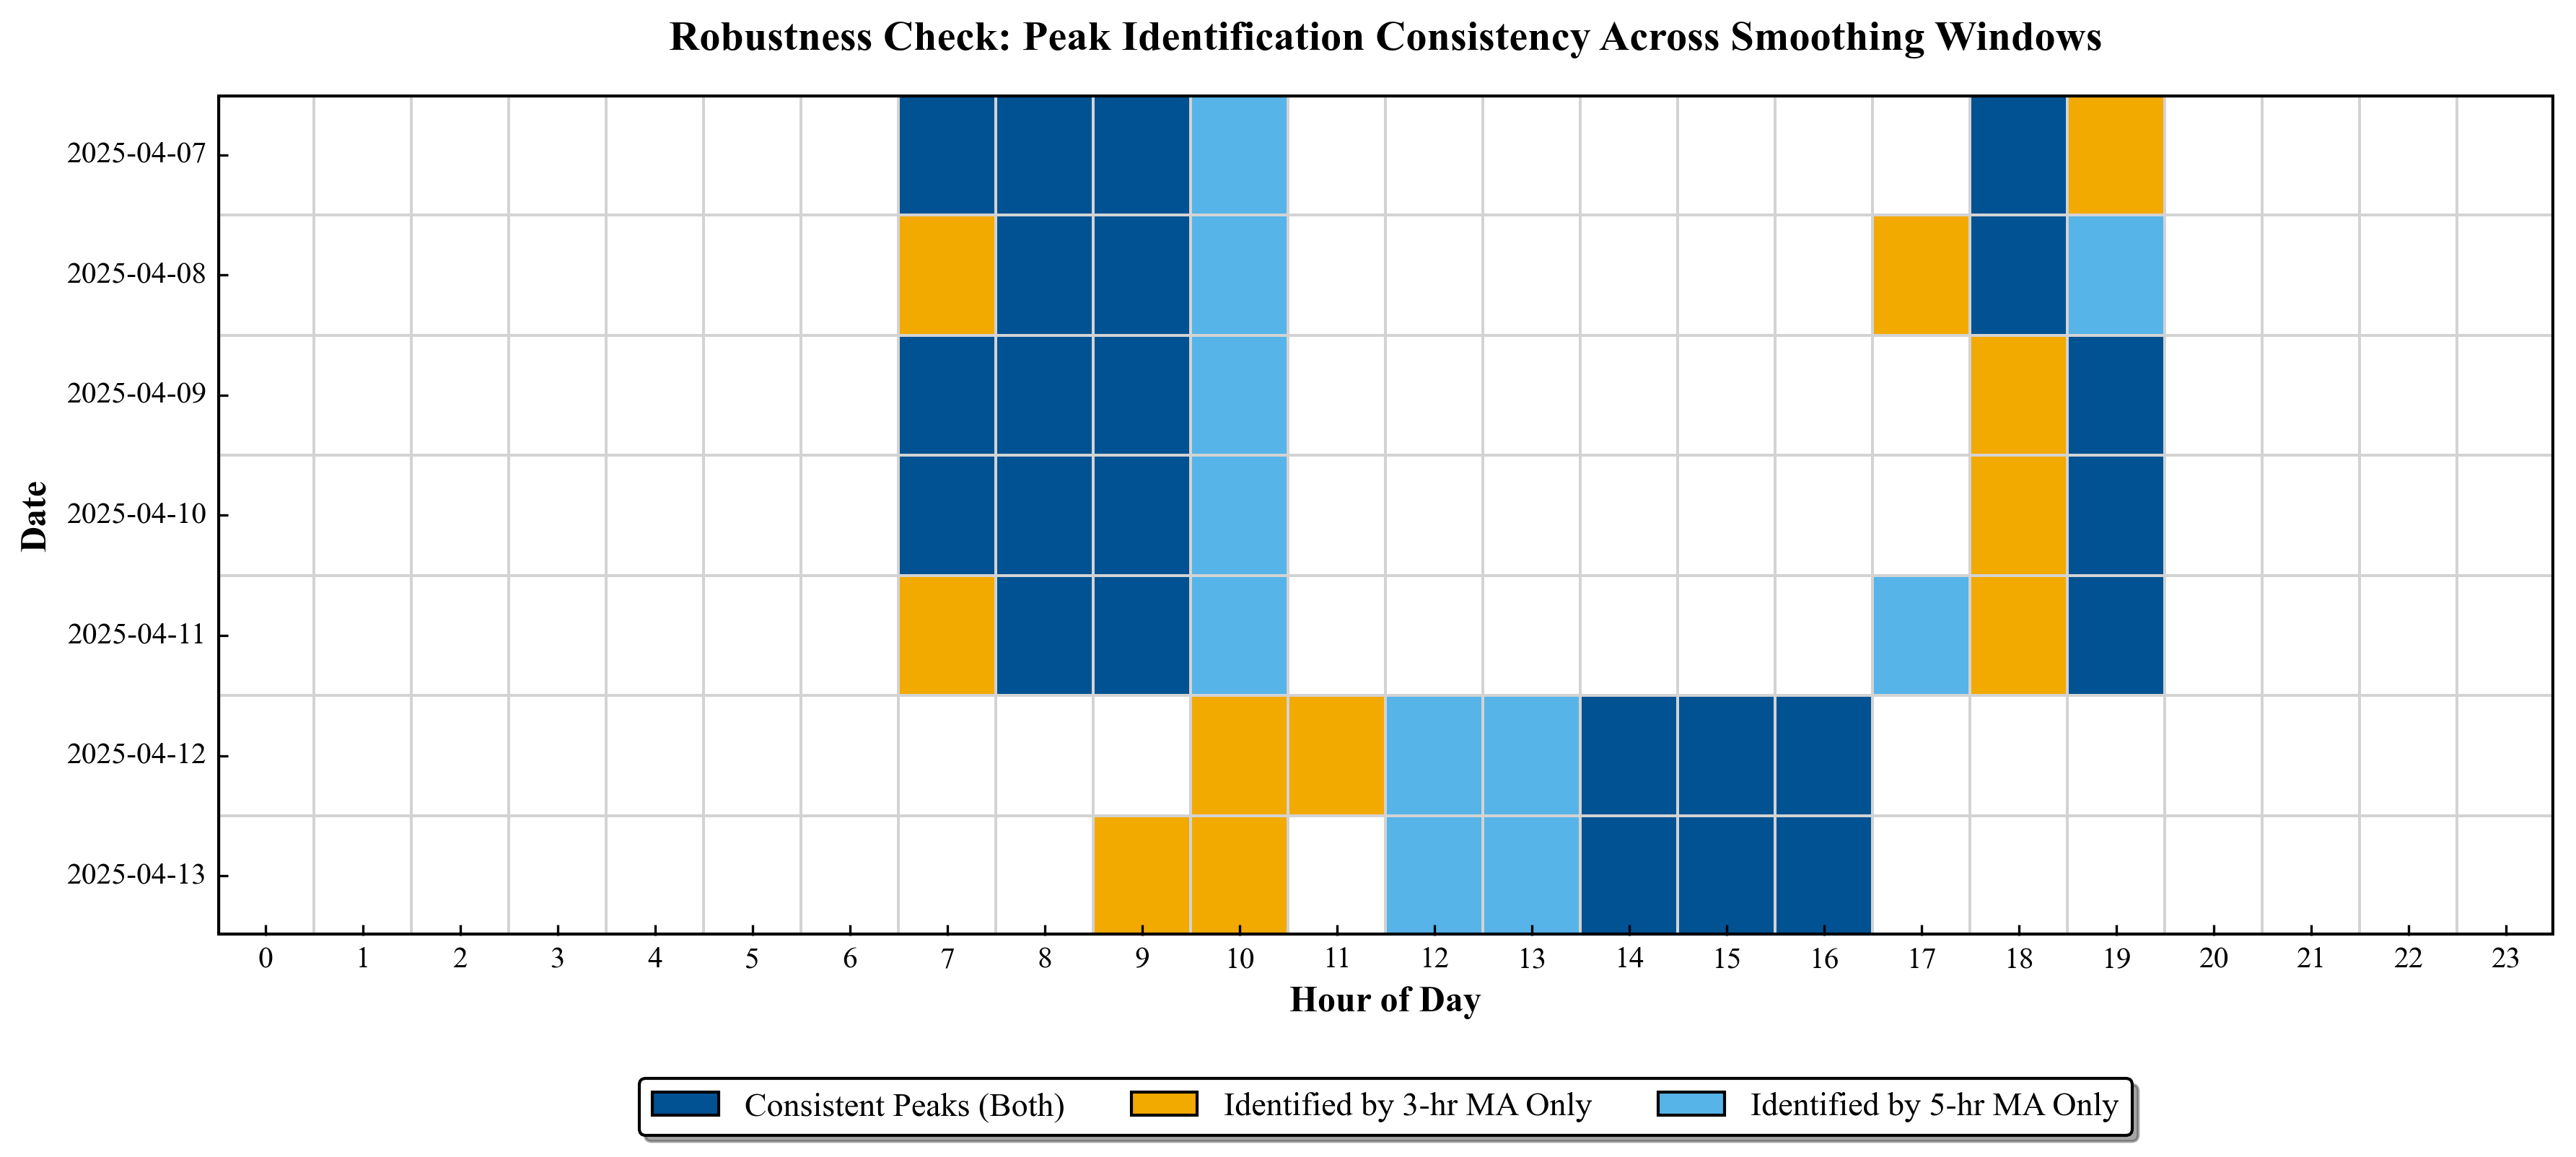
\includegraphics[width=0.9\textwidth]{Fig4_Robustness.png} 
    \caption{稳健性检验：不同平滑窗口尺度下高峰判定的重合度与差异矩阵}
    \label{fig:robustness}
\end{figure}

交叉验证的结果令人信服。由图 \ref{fig:robustness} 可见，尽管窗口尺度的改变在个别边缘时段（浅色区块）引发了微小的判定偏移，但整个系统核心的早晚高峰区块（深蓝色区块）呈现出了极高的刚性重合度。这种结构层面的高度一致性，强有力地证明了由本节双重阈值模型锁定出的“双峰潮汐特征”是区域需求的客观内在属性，而绝非数据平滑操作带来的人为假象。本模型的高峰判定标准对参数扰动具有优异的稳健性。




















\subsubsection{极端借还站点的时空分布特征挖掘}

在明确了宏观的时间高峰后，单车供需的时空错配往往在特定的“极热”与“极冷”站点表现得尤为突出。为了精准刻画这种错配特征，本文基于多源数据映射，对服务端点进行了深度的时空联动挖掘。

\textbf{1. 基于 POI 映射的空间特征定性分析}

为了避免主观臆断并增强结论的可解释性，本文提取了附件 1 中各站点的地理编码与命名属性，并结合高德地图 POI 语义特征，将大学城及周边 30 个站点严格映射为四大功能核心区：文教科研区、商业与交通枢纽区、居住生活区以及休闲与公共设施区。

随后，本文计算了全周总借出量，筛选出吞吐量极其庞大的 Top 5 站点（极热）与需求极度萎靡的 Bottom 5 站点（极冷）。为了直观展现这批极端站点的空间集聚态势，本文引入了 Voronoi 泰森多边形算法对站点的辐射服务面积进行了空间分割，并叠加了借出量气泡层（如图 \ref{fig:spatial_voronoi} 所示）。

\begin{figure}[H]
    \centering
    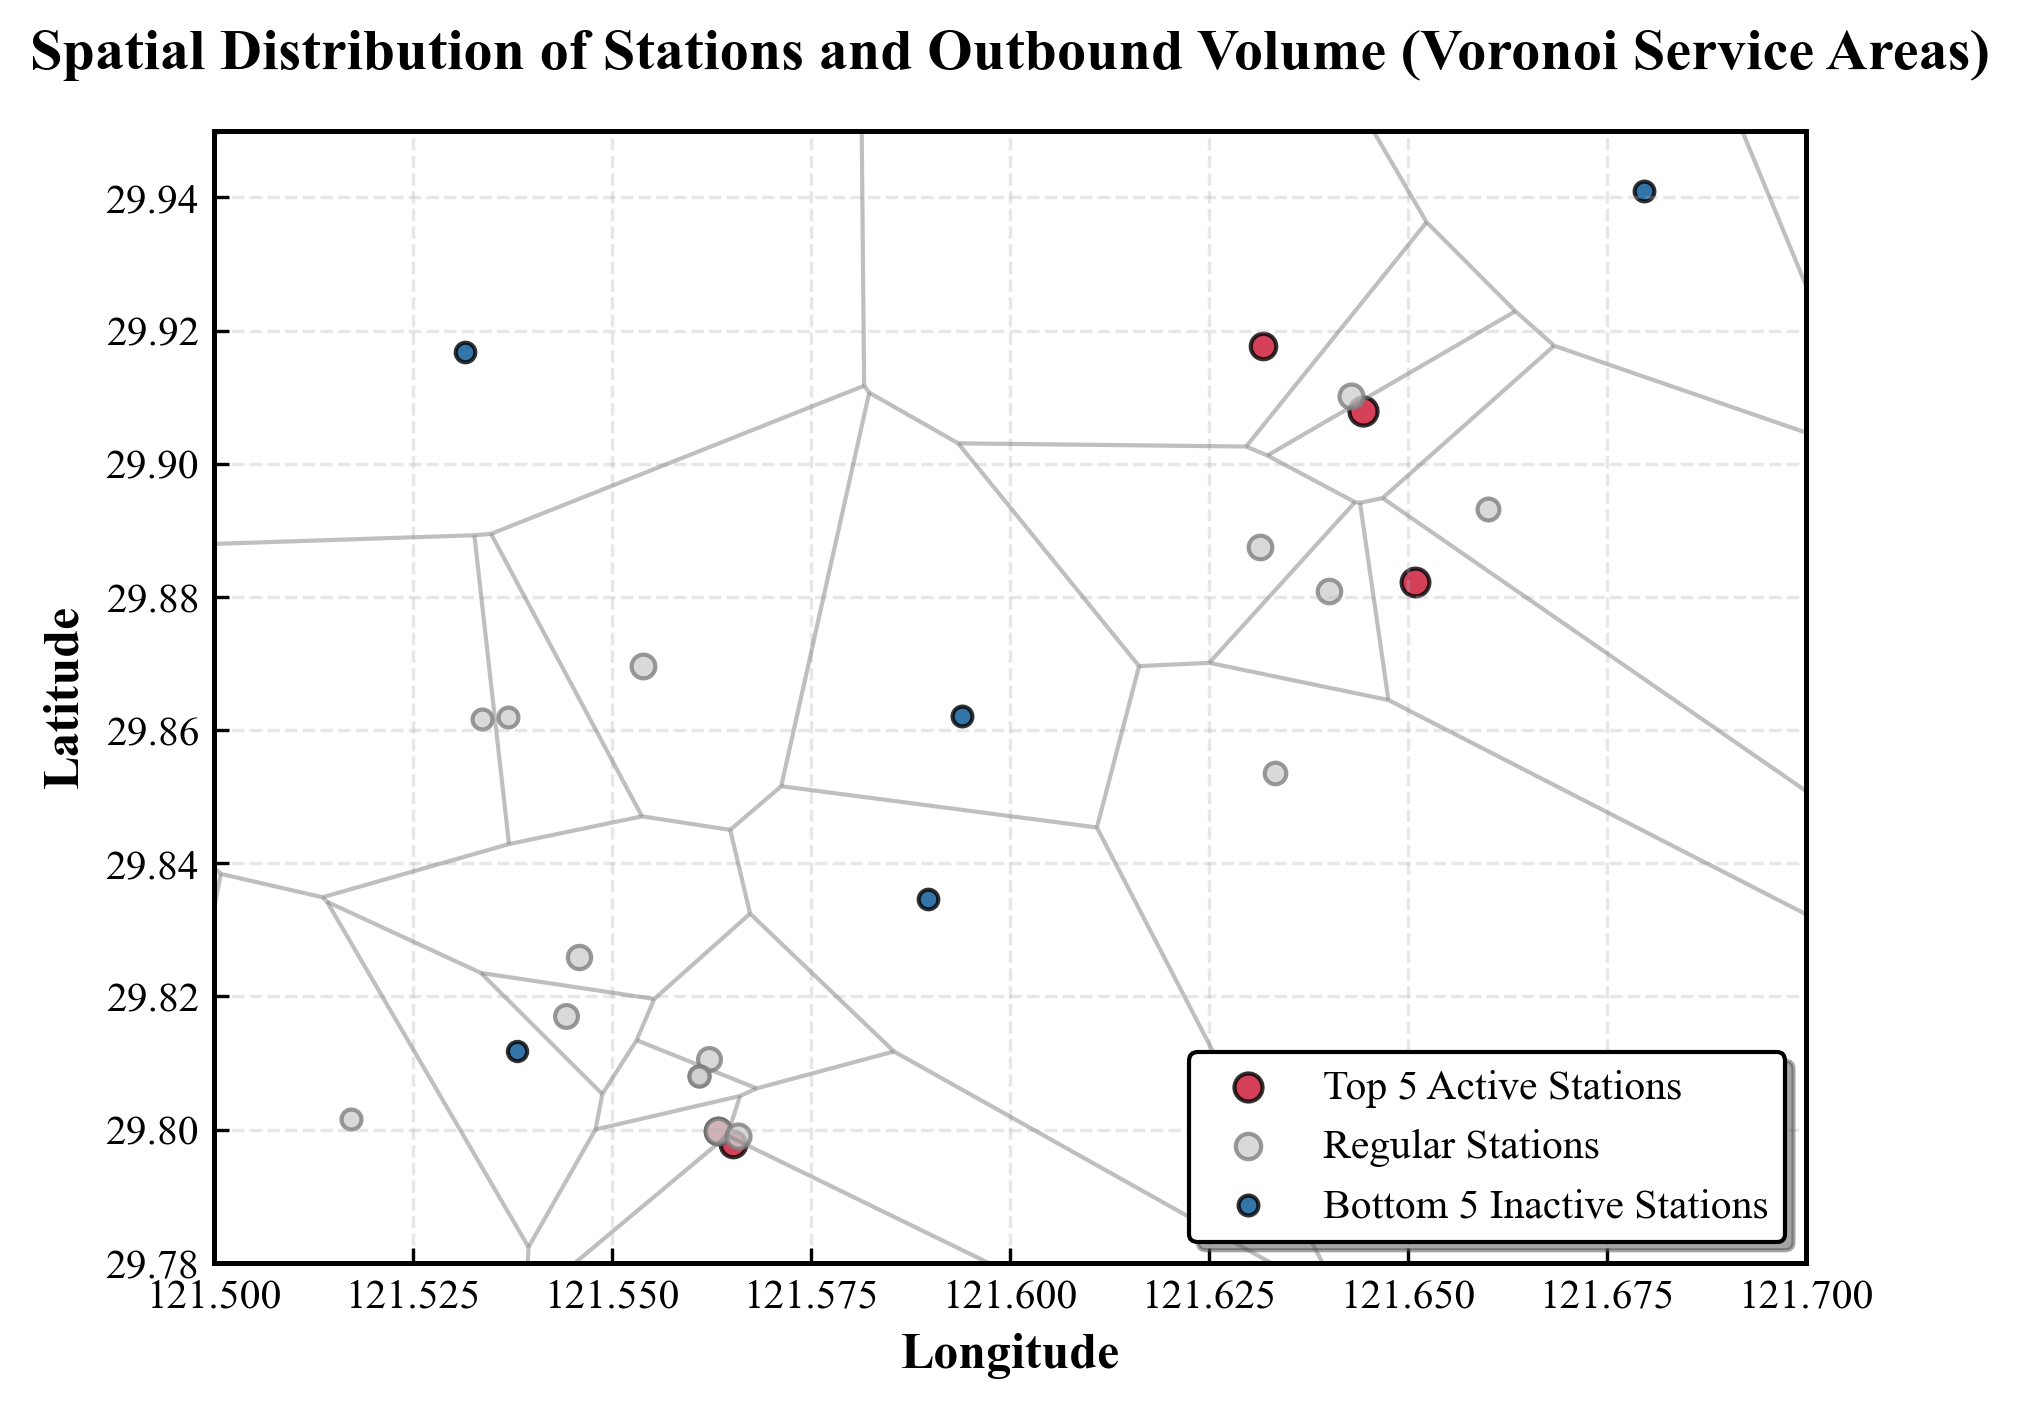
\includegraphics[width=0.9\textwidth]{Fig5_Spatial_Voronoi.png} 
    \caption{单车站点基于 Voronoi 分割的空间分布及 Top/Bottom 5 规模气泡图}
    \label{fig:spatial_voronoi}
\end{figure}

空间分布图揭示了显著的聚集规律：Top 5 极热站点无一例外地高度重叠于“商业与交通枢纽区”及“文教科研区”的黄金交界处（尤其是紧邻地铁站与核心教学区），具备极强的虹吸效应；而 Bottom 5 极冷站点则零星散布在“休闲与公共设施区”等系统边缘节点，因缺乏硬性的通勤支撑而导致车辆长期闲置。

\textbf{2. 潮汐相位与不对称性的时间特征定量分析}

空间的高客流并不会直接导致“无车可借”或“车辆积压”，真正的痛点在于极端站点内部借与还\textbf{“潮汐相位不对称性（Tidal Asymmetry）”}。

本文进一步提取了 Top 5 极热站点的日内时序均值（如图 \ref{fig:tidal_asymmetry} 所示）。数据清晰地勾勒出了这种错位现象：在早高峰（7:00-9:00）期间，借出量呈现断崖式的飙升，而归还量却处于极低水平，形成了巨大的“净流出缺口”，这是引发“无车可借”的根本时间诱因；反之，在晚高峰（17:00-19:00），归还量又远超借出量，形成“净流入冗余”，直接导致了车辆积压与满桩惩罚。

\begin{figure}[H]
    \centering
    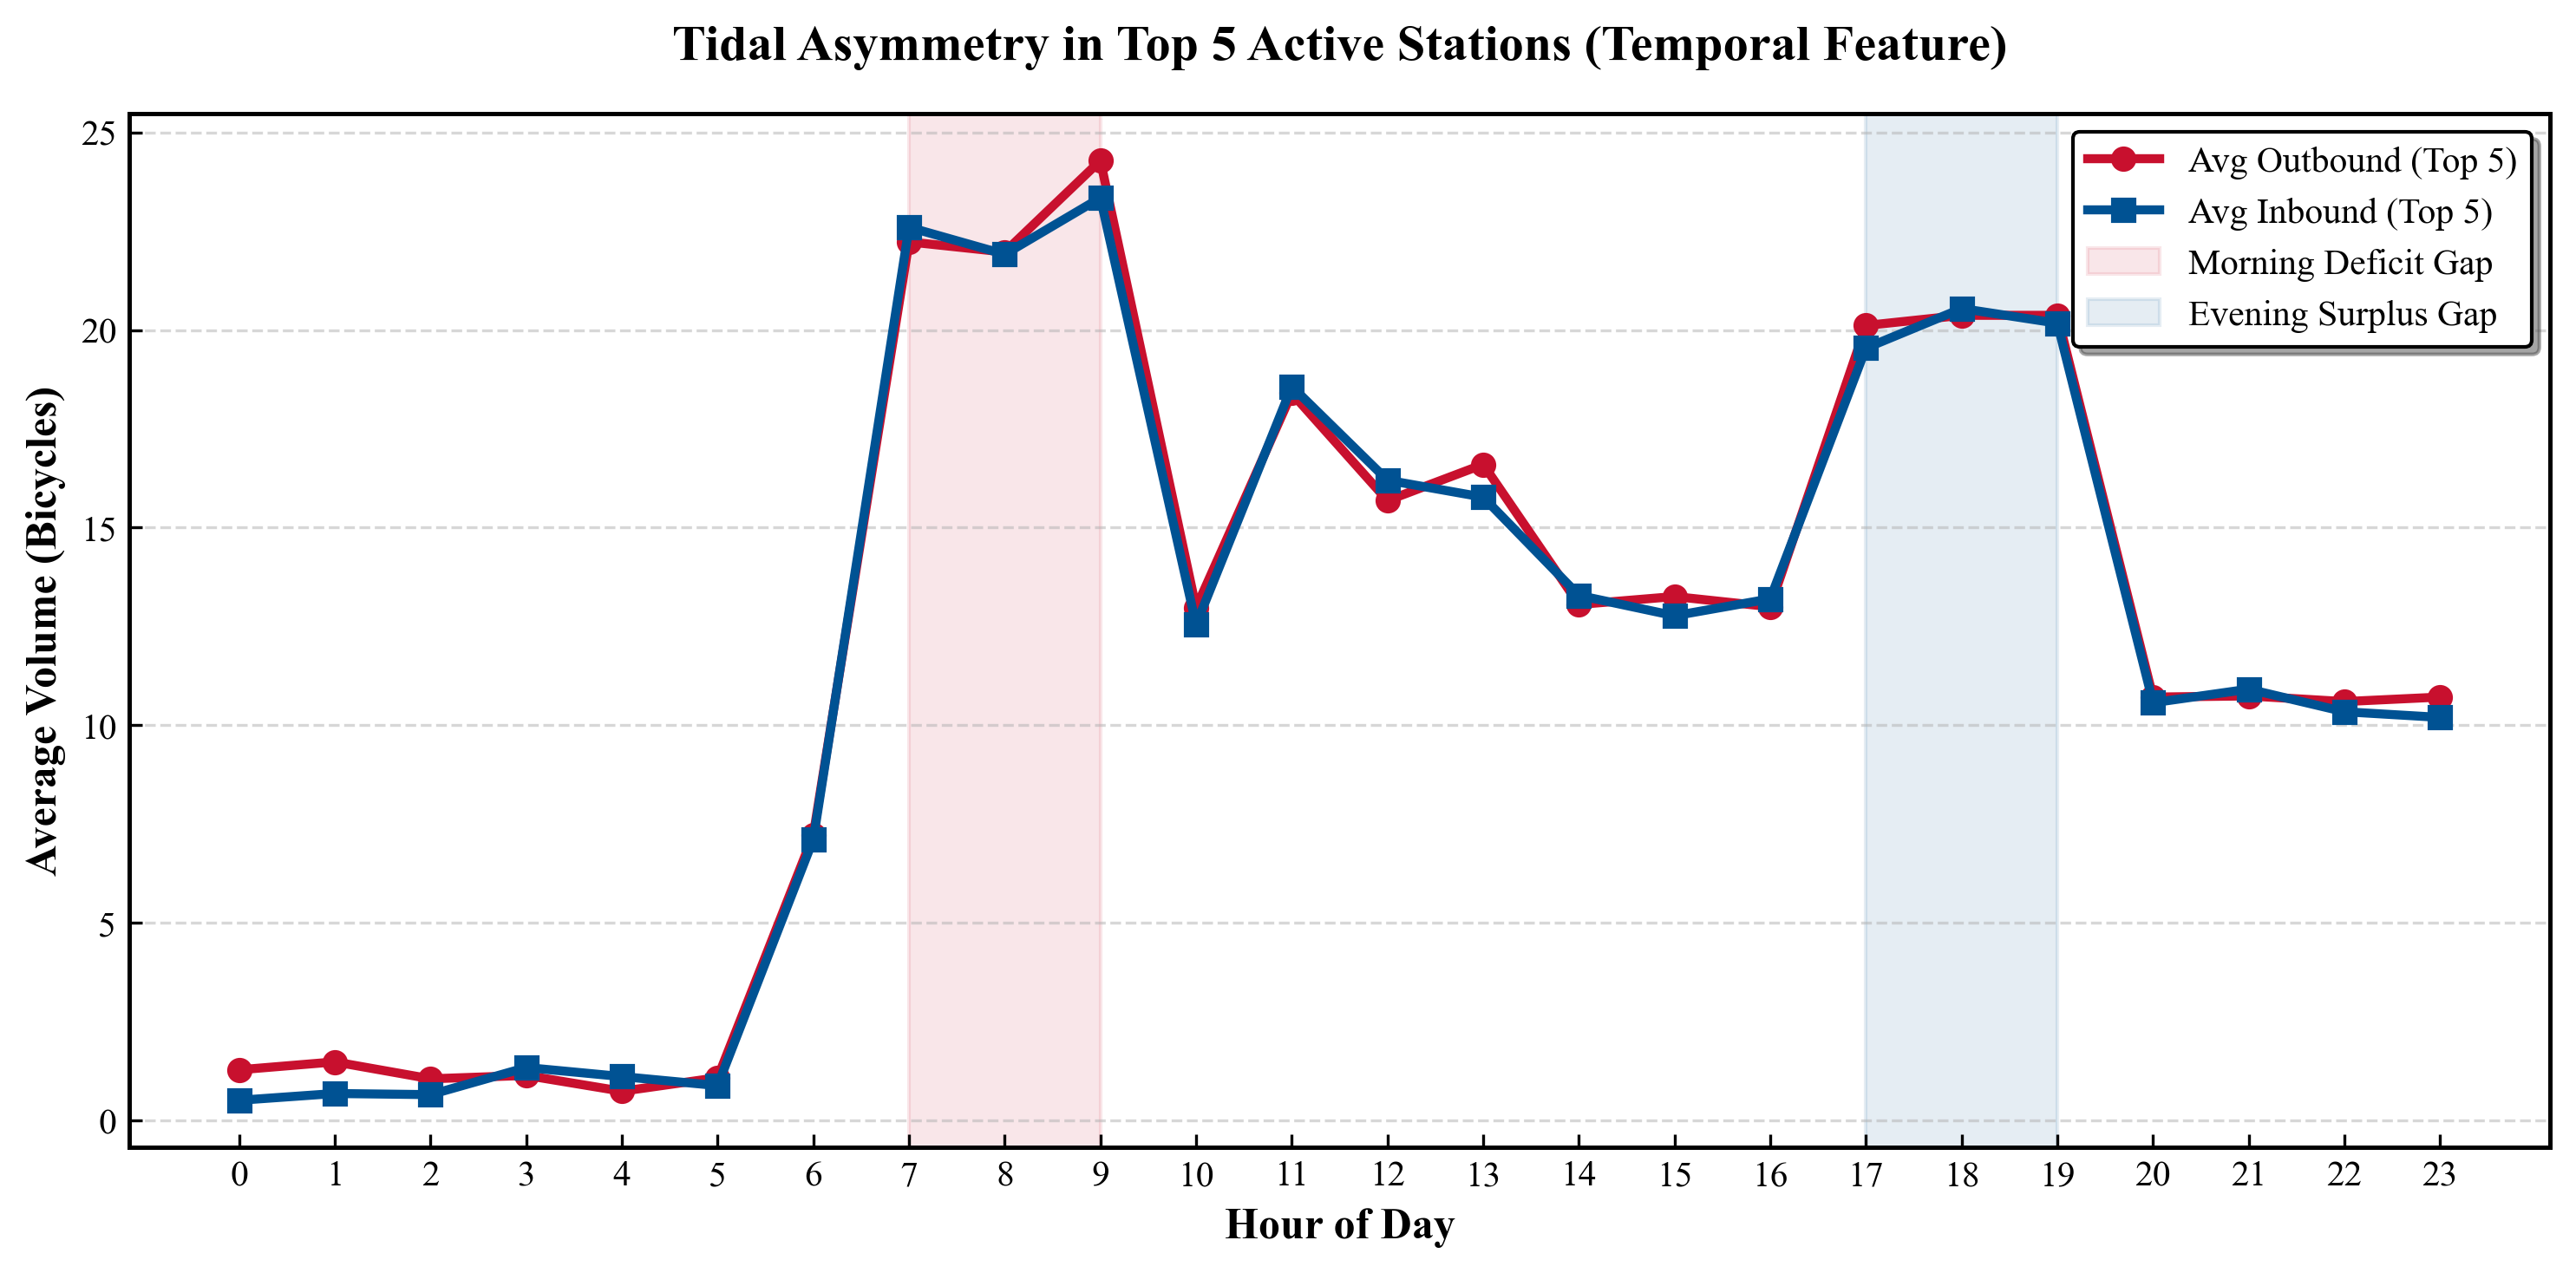
\includegraphics[width=0.9\textwidth]{Fig6_Tidal_Asymmetry.png} 
    \caption{Top 5 极热站点借出与归还需求的时序错位与潮汐不对称现象}
    \label{fig:tidal_asymmetry}
\end{figure}

这种定量与定性相结合的特征挖掘，将复杂的供需矛盾抽象成了明确的时序缺口指标，为第三问中构建以“平衡供需与成本极小化”为目标的运筹约束矩阵指明了方向。

\paragraph{稳健性检验：评估维度的多元化验证}

前文基于“单周总借出量”筛选极端站点的方法虽然直观，但从统计学严谨性角度考量，存在两处潜在的评估盲区：其一，总借出量可能受单周内某几个偶发极值日主导，未必能反映常态化的极热规律；其二，由于不同站点的总桩位容量（$C_s$）存在客观差异，单纯比较绝对吞吐量极易引发“规模偏差”，从而高估大容量站点的实际热度。

为排除上述干扰，本文针对极端站点的识别引入了另外两个维度的评估指标进行稳健性检验：
\begin{itemize}
    \item \textbf{时间频次维度（Sens 1）}：统计全周 7 天内，某站点进入日借出量 Top 5 或 Bottom 5 的总天数（即 $N^{top5}_{s}$ 与 $N^{bottom5}_{s}$），以筛选出稳定且持续的极端站点。
    \item \textbf{相对强度维度（Sens 2）}：引入单位桩位借出强度指标 $\eta_s = \frac{B_s^{total}}{C_s}$，通过消除物理容量的基数差异，刻画站点的真实周转效率。
\end{itemize}

本文分别计算了全区 30 个站点在基础模型（总借出量）、频次维度与强度维度下的全区排名，并绘制了排名演变轨迹图（如图 \ref{fig:rank_robustness} 所示）。

\begin{figure}[H]
    \centering
    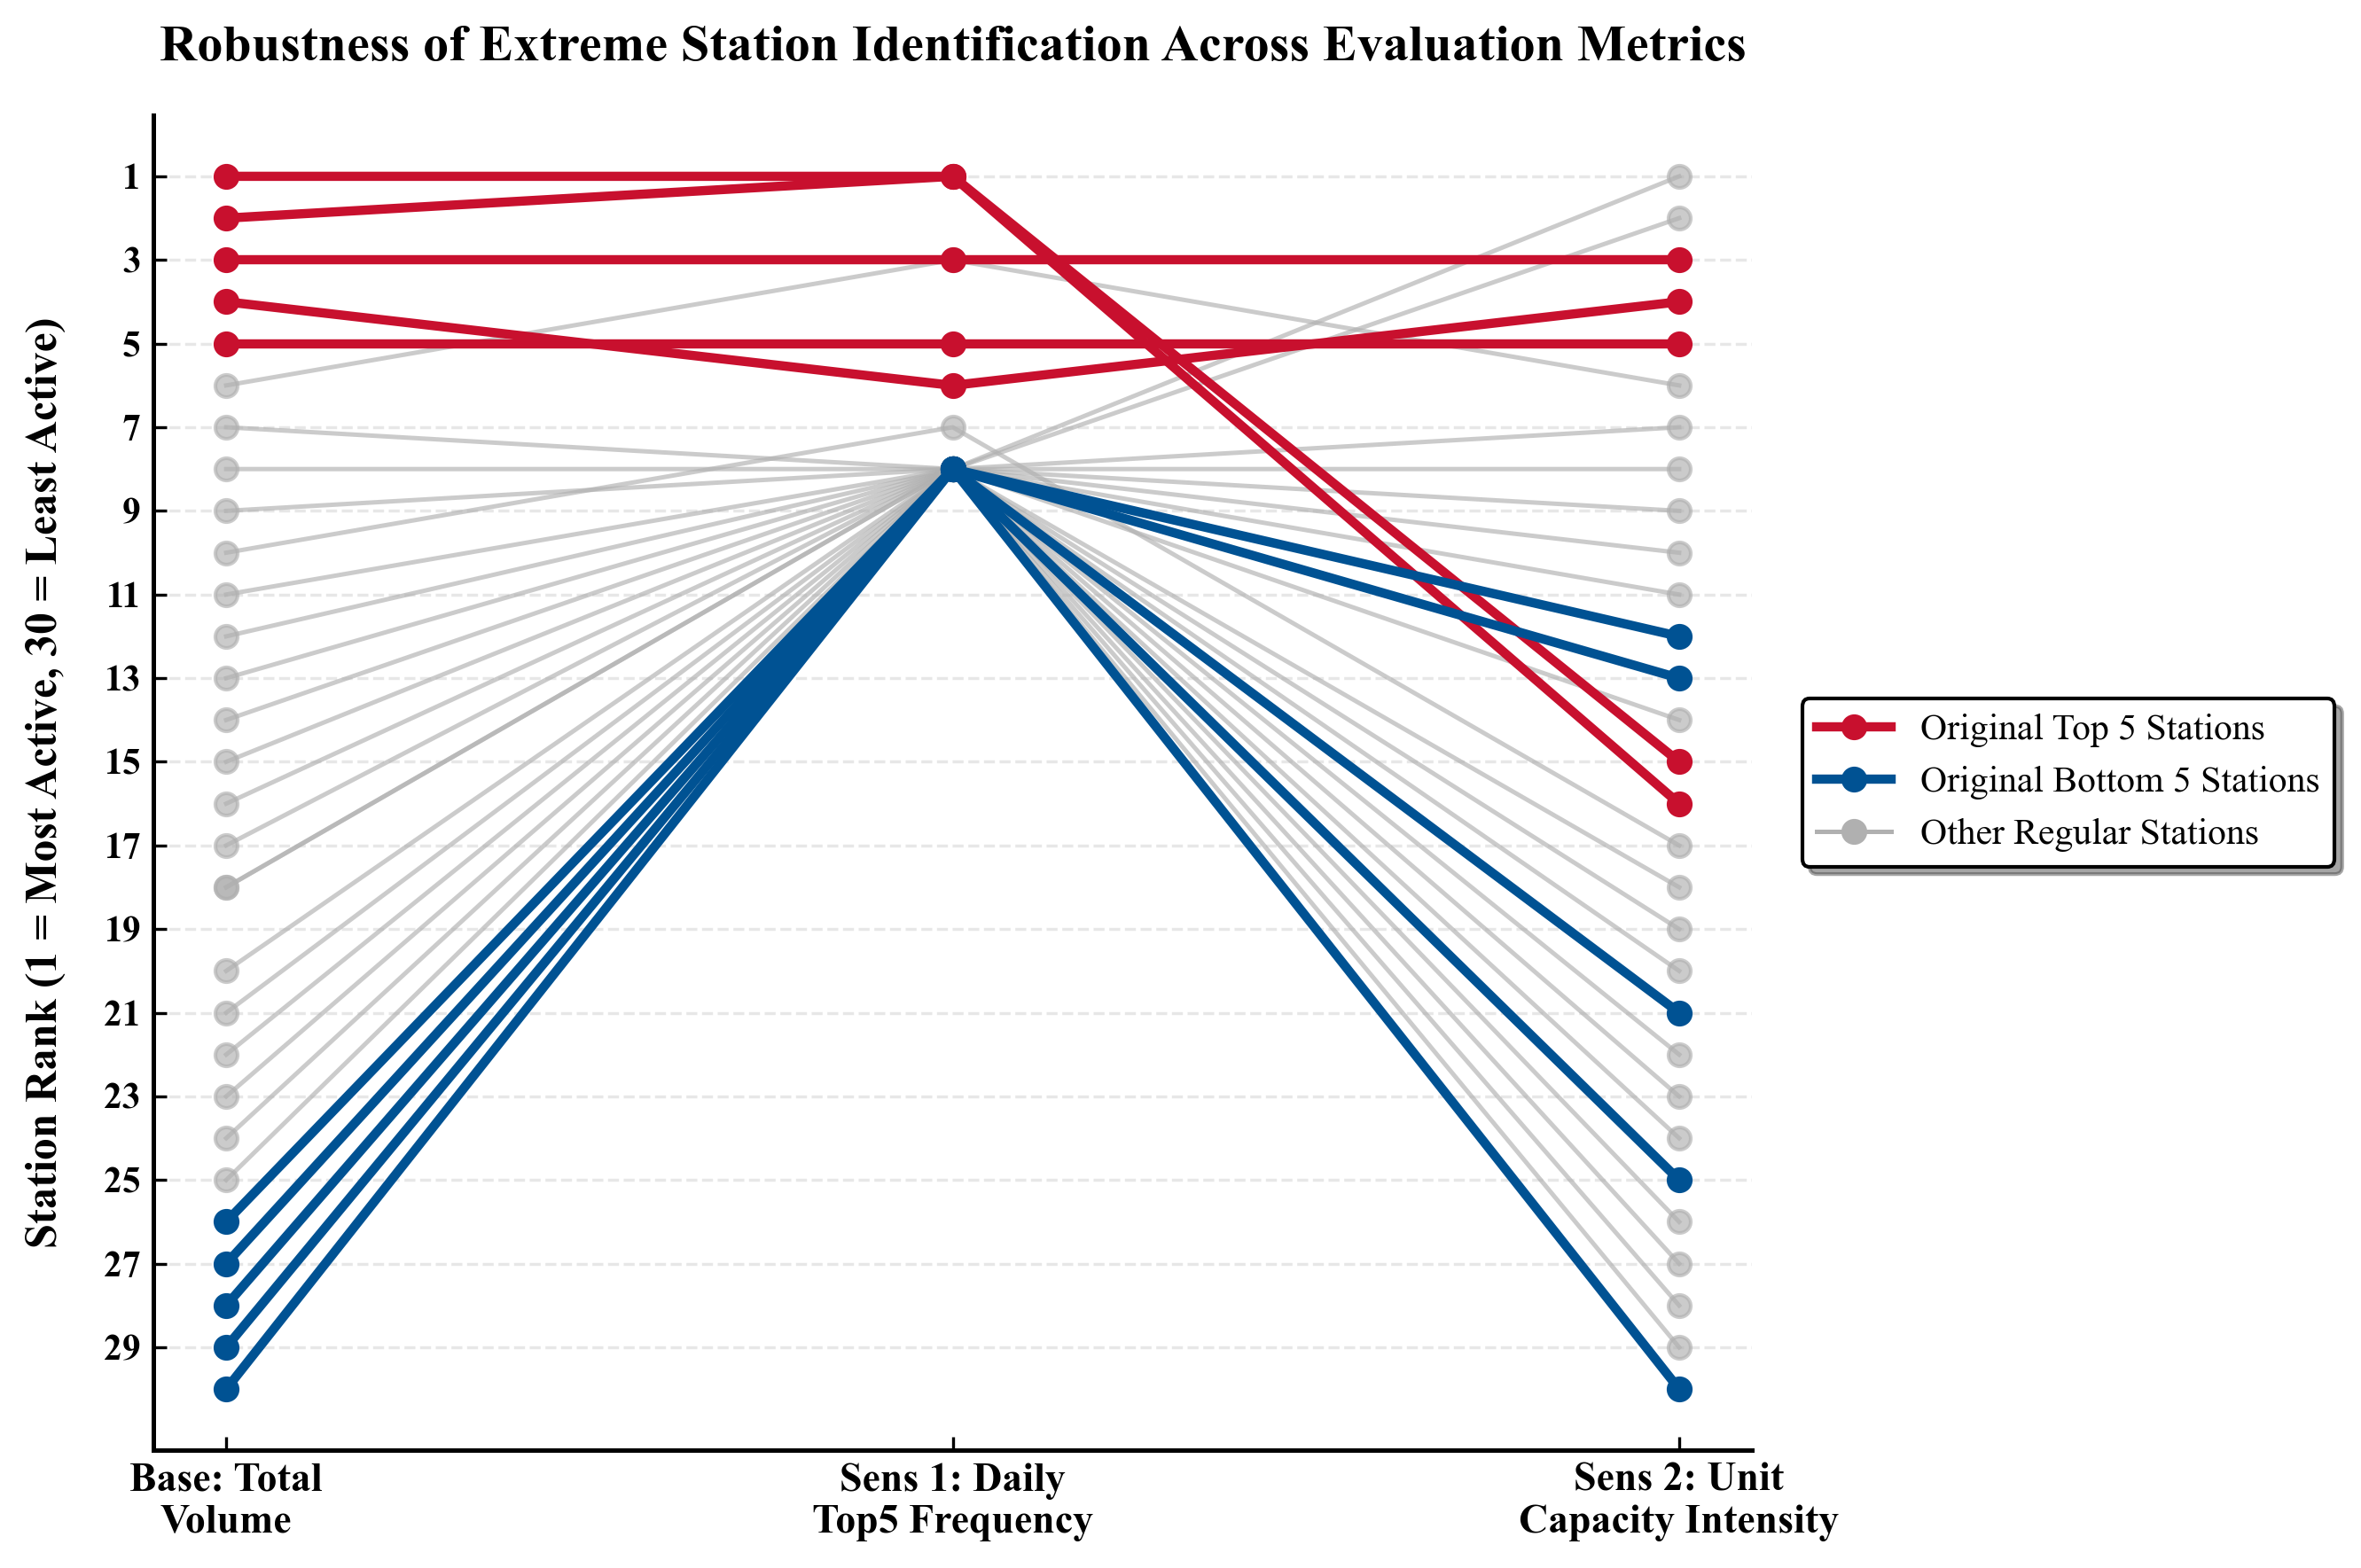
\includegraphics[width=0.85\textwidth]{Fig7_Rank_Robustness.png} 
    \caption{稳健性检验：核心极端站点在多元评估维度下的排名演变轨迹}
    \label{fig:rank_robustness}
\end{figure}

交叉验证结果显示，尽管评估标准发生了根本性重构，基础模型识别出的原始 Top 5（图 \ref{fig:rank_robustness} 中红色高亮轨线）与 Bottom 5（蓝色高亮轨线）站点的排名轨迹始终平行黏附于全区的前列与末尾，未出现明显的排名断层或交叉跌落。这一高度一致的结构刚性，确凿地证明了本文所定位出的“时空极端节点”是整个路网拓扑中客观存在的潮汐痛点，结论具备极强的抗干扰性与稳健性。

\subsubsection{工作日与休息日借还模式的差异化对比}

共享单车的骑行需求是城市居民作息规律的直接镜像。由于工作日与休息日的出行目的（硬性通勤 vs 弹性休闲）存在本质区别，本节将从“宏观城市级”与“微观站点级”双重视角出发，对两类日期的借还模式进行深度量化对比验证。

\textbf{1. 宏观城市级分布差异与统计学显著性检验}

在城市全局宏观尺度下，本文聚合了全区站点的小时级总吞吐量。为了严谨判定工作日与休息日的时序数据是否在分布形态上存在根本性差异，考虑到单车需求数据具有显著的长尾右偏特性（不符合正态分布），本文摒弃了常规的独立样本 t 检验，转而执行对非正态数据更具鲁棒性的 \textbf{Mann-Whitney U 非参数检验}。

\begin{figure}[H]
    \centering
    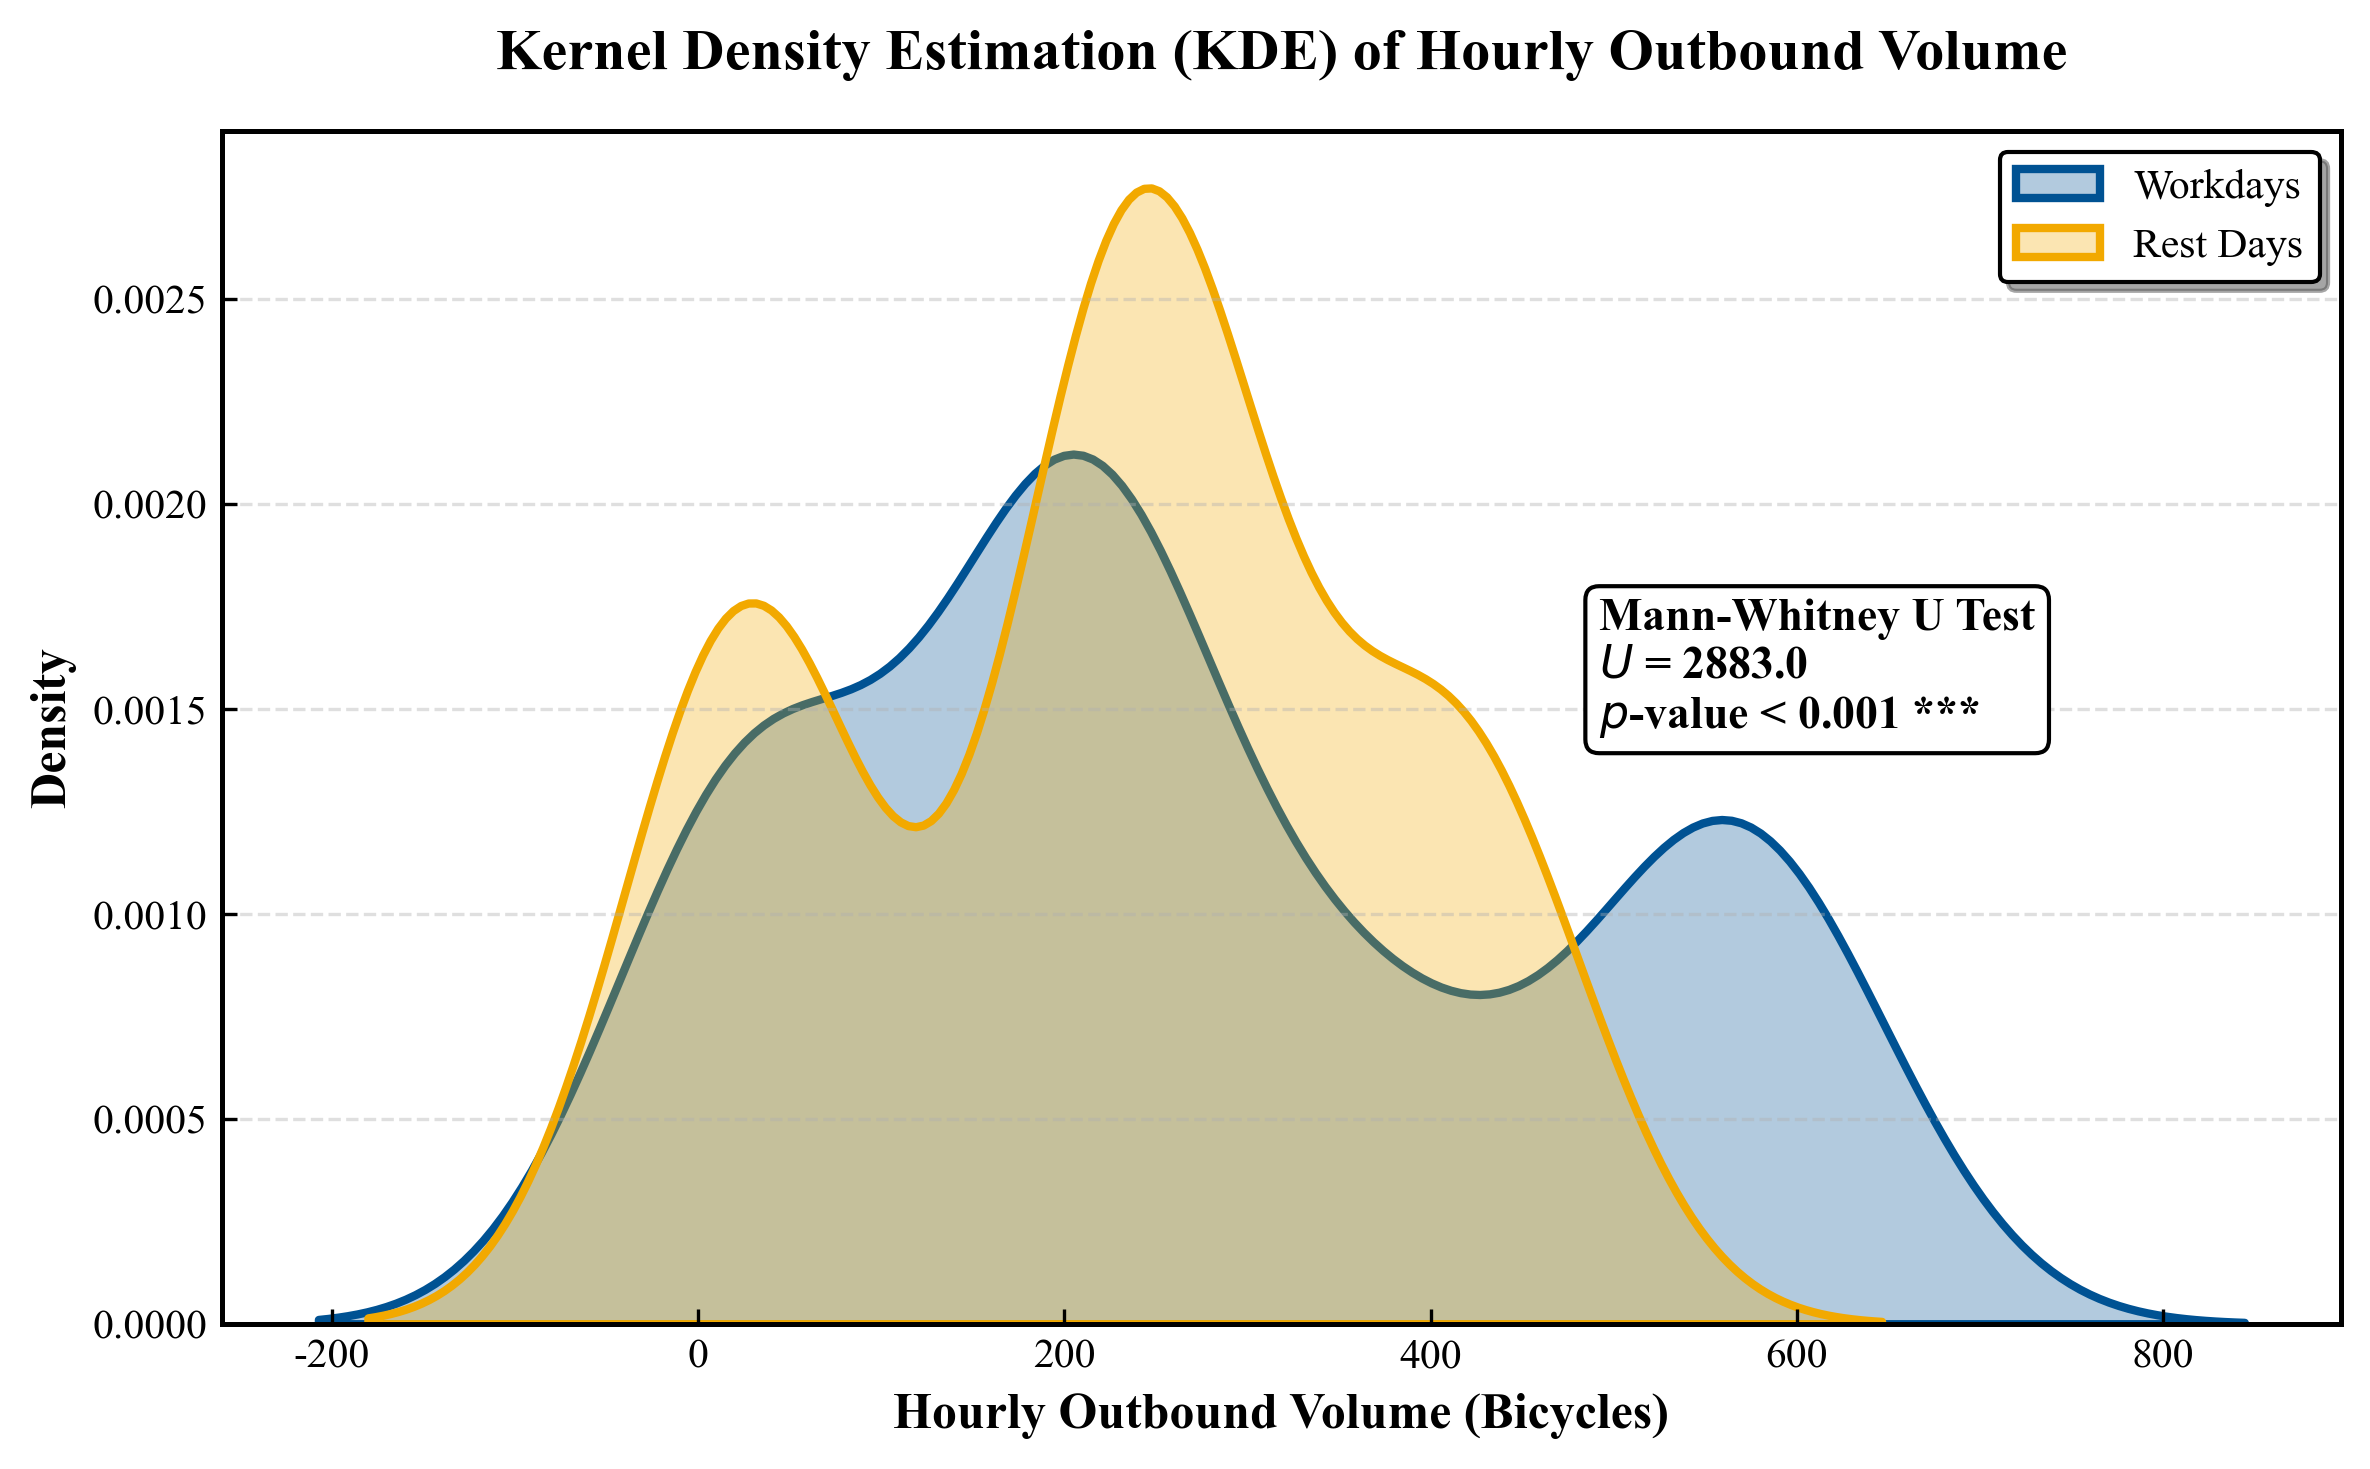
\includegraphics[width=0.85\textwidth]{Fig8_KDE_Test.png} 
    \caption{宏观城市级全天借出需求核密度估计（KDE）与 Mann-Whitney U 检验显著性}
    \label{fig:kde_test}
\end{figure}

如图 \ref{fig:kde_test} 所示，全天借出量的核密度估计（KDE）曲线揭示了两类日期截然不同的波峰形态。检验结果显示 $p\text{-value} < 0.001$，在 1\% 的显著性水平下，拒绝了工作日与休息日分布相同的原假设，在严苛的统计学意义上确证了两者借还模式的根本性异质性。

同时，宏观指标对比（图 \ref{fig:macro_micro}a）进一步佐证了这一结论：休息日的整体均值与最大值均出现断崖式下跌，表明整体需求急剧萎缩；但值得注意的是，休息日的变异系数（CV）显著低于工作日。这说明工作日的单车流转在日内经历了剧烈的脉冲式震荡（如极端的早晚高峰），而休息日的需求则在全天保持相对平缓的缓释状态。

\begin{figure}[H]
    \centering
    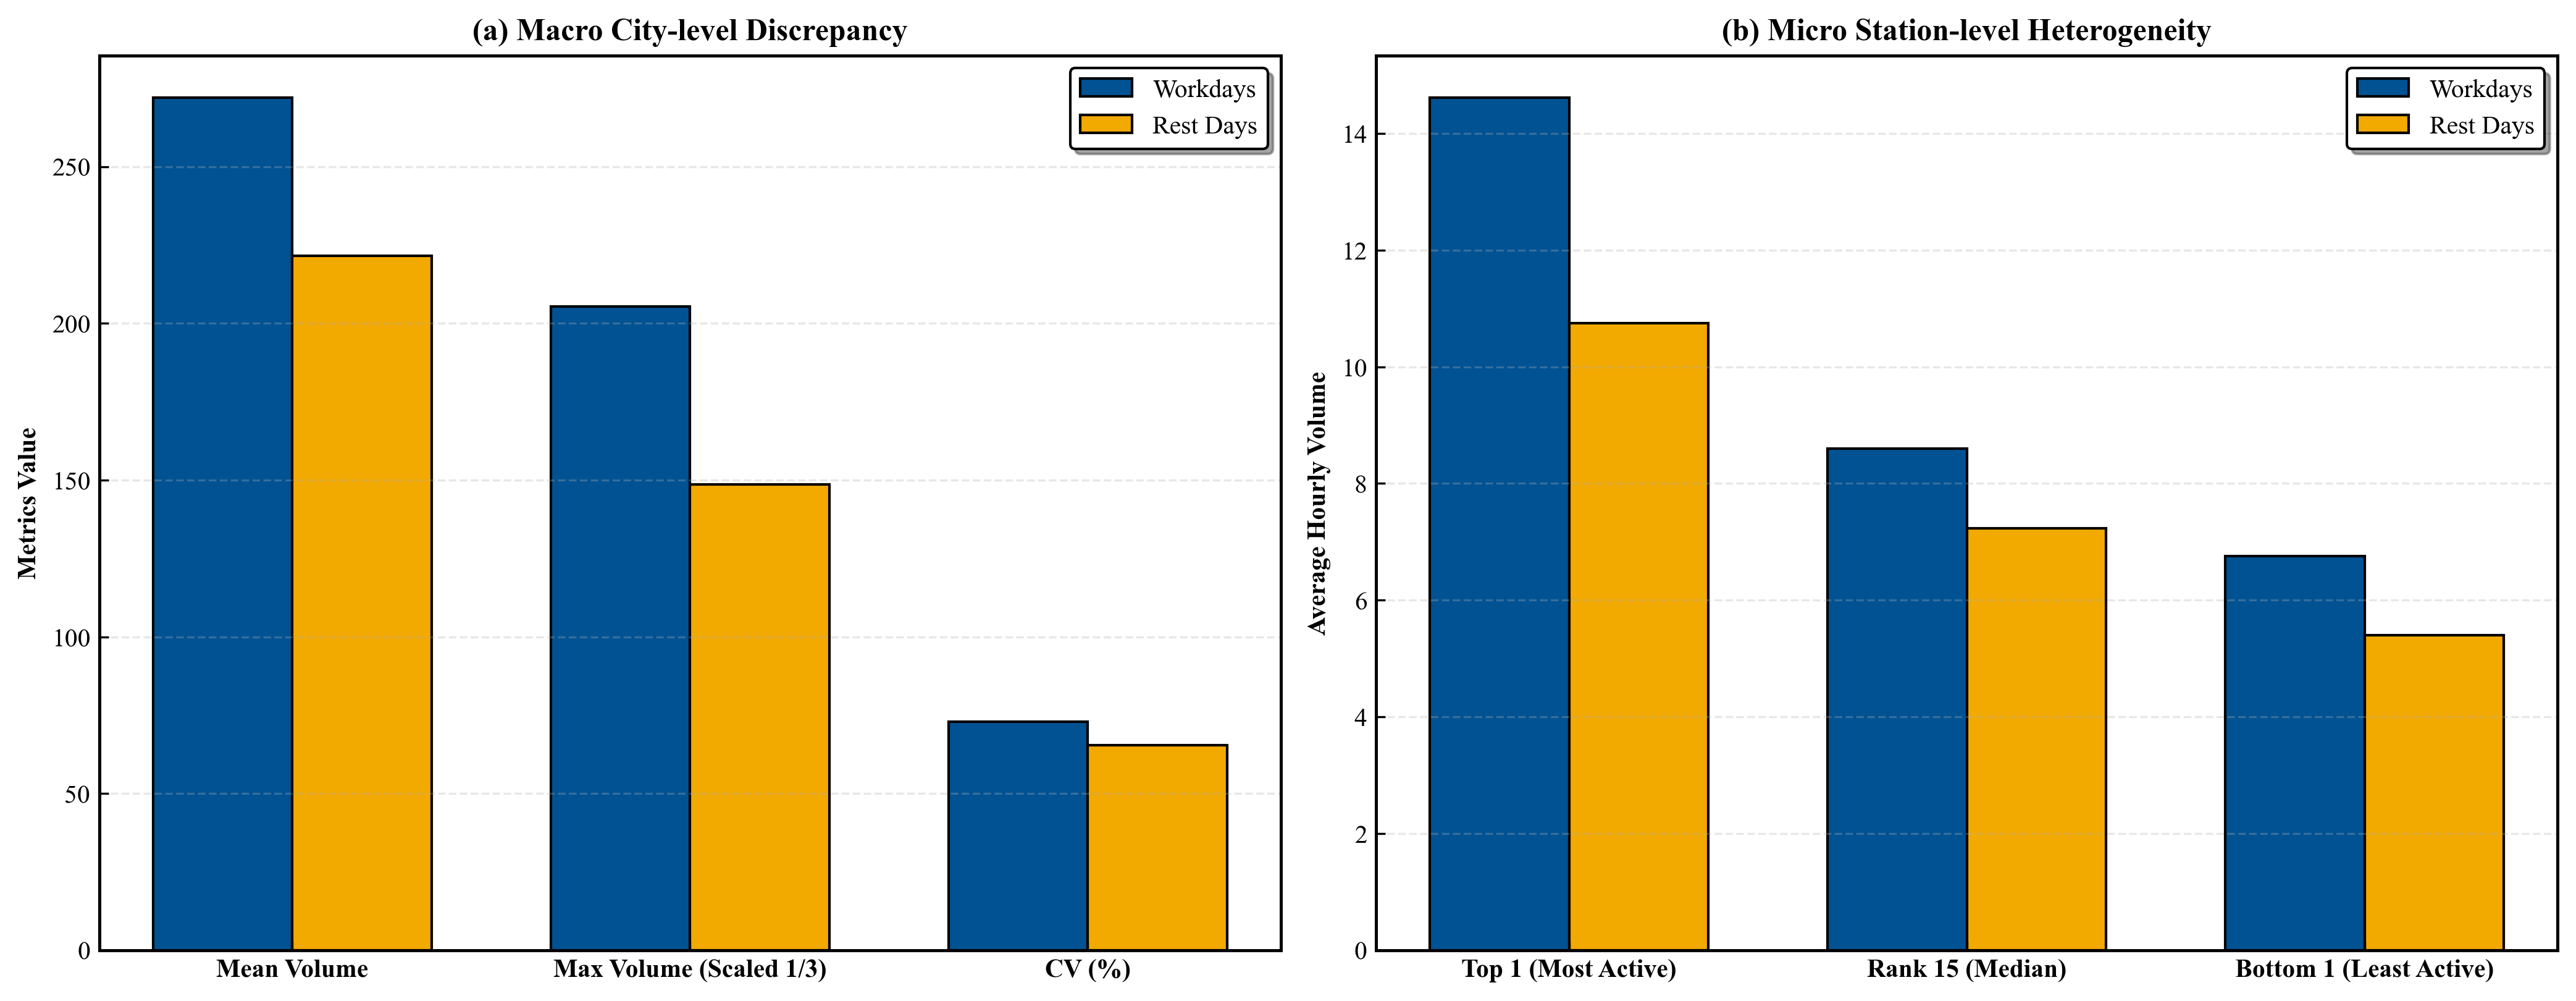
\includegraphics[width=0.95\textwidth]{Fig9_Macro_Micro_Bars.png} 
    \caption{工作日与休息日宏微观指标对标：(a) 城市级整体波动 (b) 站点级异质性}
    \label{fig:macro_micro}
\end{figure}

\textbf{2. 微观站点级异质性与“错峰延时”特征挖掘}

在微观尺度下，均值掩盖了个体特征。本文特意抽取了具有代表性的三个节点：全区总借出量 Rank 1（极热站点）、Rank 15（中位数站点）与 Rank 30（极冷站点）进行截面扫描。从图 \ref{fig:macro_micro}b 可以看出，热度越高的站点，其受作息切换带来的“潮汐衰退”冲击越猛烈；而原本低热度的极冷站点，在两类日期中始终保持死水微澜的状态，几乎不受工作日效应影响。

除了绝对数量的衰退，休息日出行中最核心的规律变迁体现在\textbf{“峰值相位的时移错位”}。本文针对 Top 1 站点的工作日与休息日日内时序轨迹进行了追踪刻画（如图 \ref{fig:time_delay} 所示）。

\begin{figure}[H]
    \centering
    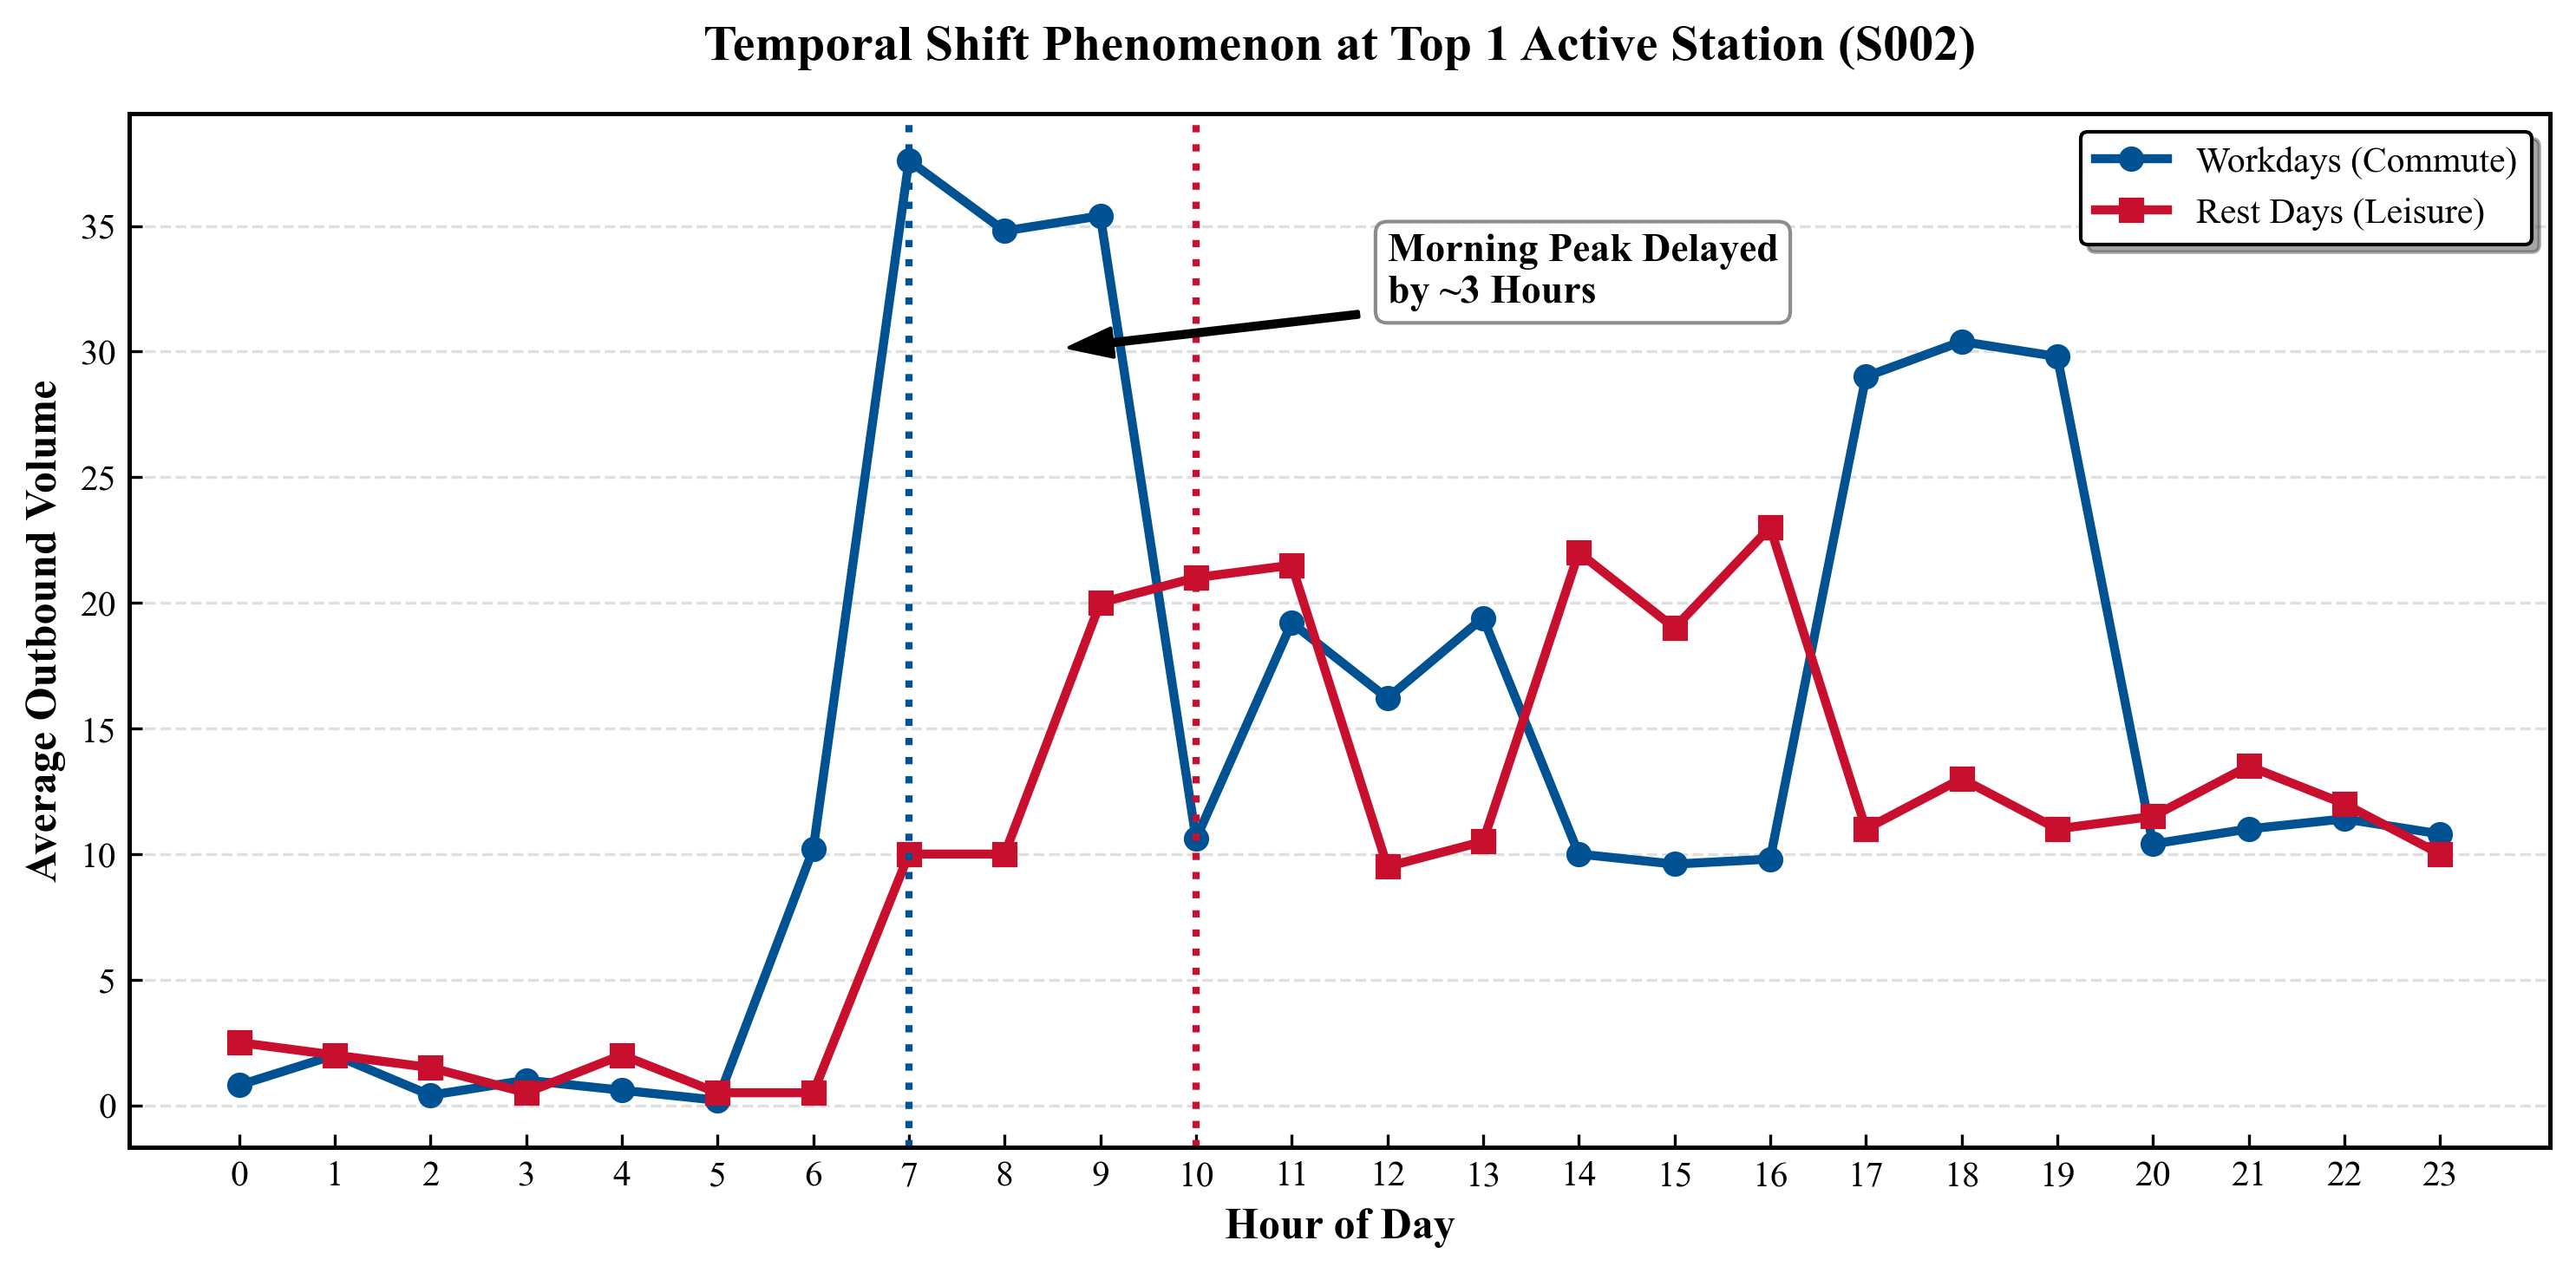
\includegraphics[width=0.85\textwidth]{Fig10_Time_Delay.png} 
    \caption{核心极热站点（Top 1）日内时序演变及早高峰“错峰延时”现象}
    \label{fig:time_delay}
\end{figure}

追踪结果表明，伴随通勤刚需的消退，休息日的早高峰不仅在强度上被极大削弱，其波峰到达时间也发生了显著的\textbf{“错峰延时（Time Delay）”现象}：原先由于赶早八课程或早高峰打卡而在 7:00 骤然爆发的早高峰，在休息日平缓地推迟了近 3 个小时（延宕至上午 10:00 左右）才缓慢达到温和的日内高点。

这种对“工作日激进脉冲”与“休息日延时缓释”的双轨制时空模式识别，对后续建模至关重要。它提示我们在解答第二问与第三问时，绝不能用一套静态的参数去约束整个系统，而必须针对日期属性构建动态的需求预测引擎与自适应的时间窗调度策略。

\subsection{问题二：基于历史时序数据的需求预测模型} 
（说明预测模型的原理、特征工程、评价指标，展示测试集预测结果及三张代表性站点的预测曲线与实际值对比图。）

\subsection{问题三：最小化总费用的运筹调度优化模型} 
（基于离散时间步构建混合整数规划模型，写明目标函数及空/满桩惩罚等约束条件。设计求解算法，给出最优调度路线与时间表，并量化对比调度前后的日总费用及用户无法借还车次数。分析调度方案对用户需求率的影响及平衡策略。）


\section{模型推广与灵敏度分析（问题四）} 
% （注：将原先的“结果分析与检验”替换为此章节，完美承接问题四的要求）

\subsection{空间网络拓扑的拓展适用性分析}
（响应问题四第一小问：设定新增的 5 个站点的位置及容量，说明如何将其作为新节点无缝接入问题三建立的图网络拓扑与距离矩阵中，并展示调整后的模型求解结果。）

\subsection{调度成本参数的灵敏度分析}
（响应问题四第二小问：对运输成本单价、满/空桩惩罚系数进行梯度摄动。绘制目标函数值与关键决策变量随参数变化的灵敏度曲线，剖析成本结构变化对最优调度方案（如车辆出车频次、装卸总量）的实质性影响，为运营方提供动态定价环境下的策略建议。）

\section{模型评价与改进} 
\textbf{模型优点：}
（1）...
（2）...

\textbf{模型缺点与改进方向：} 
（1）...

% ========== 参考文献 ==========
\newpage
\begin{thebibliography}{99}
\addcontentsline{toc}{section}{参考文献}
% （按正文中引用顺序列出，参考 GB/T 7714 格式）
\bibitem{ref1} 作者. 文献标题[J]. 期刊名称, 年份, 卷号(期号): 页码.
\end{thebibliography}

% ========== 附录 ==========
\newpage
\section*{附录}
\addcontentsline{toc}{section}{附录}
（包含核心代码、额外图表、数据处理过程等。建议将主体代码上传至压缩包单独文件夹，附录中附简要说明。）

\end{document}